\documentclass{mythesis}
\usepackage{mythesis}
\usepackage{amsmath}

%package for corrections: changes are in blue
\usepackage{changes}
%\usepackage[final]{changes}


%% You can set the line spacing this way
%\setallspacing{double}
%% or a section at a time like this
%\setfrontmatterspacing{double}

%% PDF metadata
\makeatletter
\@ifpackageloaded{hyperref}{%
\hypersetup{%
pdftitle = {Studying Compressed SUSY with CMS},
pdfsubject = {Robyn Lucas' PhD thesis},
pdfkeywords = {Monojets, CMS, SUSY, LHC},
pdfauthor = {\textcopyright\ Robyn Lucas},
linkcolor = black,
citecolor=black,
urlcolor=black 
}
}{}
\definechangesauthor[name={Robyn Lucas}, color=orange]{per}
\makeatother

%% Define the thesis title and author
\title{Searches for Supersymmetry with compressed mass spectra using monojet events with the CMS detector at the LHC}
\author{Robyn Elizabeth Lucas}

%% Start the document
\begin{document}

%% Define the un-numbered front matter (cover pages, rubrik and table of contents)
\begin{frontmatter}
  %% Title
\titlepage[Imperial College London]%
{A dissertation submitted to Imperial College London\\
  for the degree of Doctor of Philosophy}

%% Abstract
\begin{abstract}%[\smaller \thetitle\\ \vspace*{1cm} \smaller {\theauthor}]
  %\thispagestyle{empty}
  This is the abstract, find me in frontmatter.tex
\end{abstract}


%% Declaration
\begin{declaration}
  I, the author of this thesis, hereby declare the material presented here 
  to be the result of my own work, except where explicit
  reference is made to the work of others.
  It has not been submitted for another qualification to this or any other university. 
  All figures labelled ``CMS'' have been sourced from CMS publications, referenced in the caption, and include those produced by the author.
  Those figures labelled ``CMS Preliminary'' have been sourced from a CMS public preliminary document or an unpublished CMS document.
  All figures taken from external sources are referenced appropriately throughout this thesis.
  \vspace*{1cm}
  \begin{flushright}
   Robyn Lucas 
  \end{flushright}
\end{declaration}


%% Acknowledgements
\begin{acknowledgements}
  % Firstly, I would like to thank my parents and family for their unwavering support and encouragement throughout my academic career.
  % Secondly, I thank my supervisors Alex Tapper and Steve Worm for their advice and guidance.
  % I also express huge thanks to the Monojet analysis team; without Phat Srimanobhas my research would not have been possible, and whose patience, help and hard work I am eternally grateful for; Sarah Malik, Shuichi Kunori and Teruki Kamon, whose discussions and guidance have been invaluable.
  % Thanks also to Michele Pioppi and Andy Rose for their patience in helping a fresh faced first year who could not code in the work on upgrade jets.
  % My friends and colleagues who kept me sane in Geneva, through all those jet calibrations; Sam and Sam, Darren, Andrew, Kenzie and Patrick you provided much needed distractions and laughs, as well as more than a little bit of help over the years.
  % Lastly, I cannot express enough thanks to my boyfriend Ed, without whom I could not have survived my PhD. 
  % His unfaltering support, both in Geneva and London, were at times the only thing that kept me going. Sorry I never found the Lucas boson!
  % Finally, I thank the STFC for providing the funding that enabled me to conduct the research presented here, and for the 15 months spent out at CERN.
\end{acknowledgements}


% %% Preface
% \begin{preface}
%   This thesis describes my research on various aspects of the \CMS
%   particle physics program, centred around the \CMS detector and \LHC
%   accelerator at \CERN in Geneva.

%   \noindent
%   For this example, I'll just mention \ChapterRef{chap:SomeStuff}
%   and \ChapterRef{chap:MoreStuff}.
% \end{preface}

%% ToC
\tableofcontents

%% Strictly optional!
\frontquote%
  {For Peter}%
  {}

\end{frontmatter}

%% Start the content body of the thesis
\begin{mainmatter}
  %% Actually, more semantic chapter filenames are better, like "chap-bgtheory.tex"
  \chapter{Introduction}
\label{chap:intro}

%\chapterquote{I may not be there yet, but I am closer than I was yesterday}
%{Unknown}

%% Note that the citations in this chapter use the journal and 
%% arXiv keys: I used the SLAC-SPIRES online BibTeX retriever 
%% to build my bibliography. There are also quite a few non-standard
%% macros, which come from my personal collection. You can have them
%% if you want, or I might get round to properly releasing them at 
%% some point myself.

\chapterquote{Everything starts somewhere, although many physicists disagree.}
{Terry Pratchet}




  \chapter{Theory and Motivations}
\label{chap:theory}

%\chapterquote{I may not be there yet, but I am closer than I was yesterday}
%{Unknown}

%% Note that the citations in this chapter use the journal and 
%% arXiv keys: I used the SLAC-SPIRES online BibTeX retriever 
%% to build my bibliography. There are also quite a few non-standard
%% macros, which come from my personal collection. You can have them
%% if you want, or I might get round to properly releasing them at 
%% some point myself.

\chapterquote{Absence of evidence is not evidence of absence.}
{Carl Sagan, 1934 - 1996}%


This chapter introduces the \ac{SM} as a gauge invariant \ac{QFT}, and gives a description of the fundamental particles and their interactions.
The shortcomings of the \ac{SM}, outlined in Section~\ref{th:BSM}, imply however that it must be an incomplete description of nature. 
A Supersymmetric extension of the SM can address many of these limitations and is described in Section~\ref{th:SUSY}. 
Particular emphasis is placed on the arguments for \ac{SUSY} with compressed mass spectra in Section~\ref{th:CMPsusy}, as this is the subject of this thesis.
The convention $c=\bar{h}=1$ is used throughout. 
The four vector indices are labelled $\mu$ and $\nu$.
The $SU(2)$ generators are labelled $i$, $j$, and $k$, while the $SU(3)$ generators are labelled $a$, $b$, and $c$.
Gravity, of order $10^{33}$ times weaker than the forces discussed in this chapter, is neglected.
The lack of any explanation of gravity within the \ac{SM} suggests its incompleteness as a total description of nature.

\section{The Standard Model of Particle Physics \label{th:sm}}

The \ac{SM} of particle physics provides a fantastically accurate description of the fundamental particles of nature and their interactions via the strong, electromagnetic, and weak forces at the electroweak energy scale.
It has proved itself incredibly robust during the first years of \ac{LHC} running. 
Many high precision measurements are consistent with their loop level \ac{SM} predictions, see Figure~\ref{fig:stairwayToHeaven}, which shows 
experiment and theory expectations agree over 6 orders of magnitude, across many different processes.
Even very rare processes have been measured to agree with their \ac{SM} predictions: the decay $B_{S}\rightarrow \mu\mu$, very sensitive to new physics processes, has been observed at the level of three in every billion decays of the $B_{S}$ meson~\cite{BSmumuCombo}.
Such tests of the \ac{SM} cement its place as one of the major successes of 20$^{\rm th}$ century physics.


\begin{figure}[htbp]
  \begin{center}
  \includegraphics[width=0.8\textwidth]{Figures/theory/SigmaNew_v0}
  \caption{Combined results from \ac{CMS} of many \ac{SM} measurements made at \ac{LHC} centre-of-mass energies of 7 and 8~\TeV, taken from~\cite{CMSpublictwiki}. Theory and experiment agree over a vast range of production cross section values, for many different \ac{SM} processes.
}
  \label{fig:stairwayToHeaven}
  \end{center}
\end{figure}

Developed in the 1960's and 1970's~\cite{PhysRevLett.19.1264,Glashow:1961tr,Salam:1968rm,Hooft1971167}, the \ac{SM} is a relativistic \ac{QFT} in which particles are excitations of fields. 
It is gauge invariant, guaranteeing its renormalizability, and contains three symmetries:
$SU(3)_{C} \times SU(2)_{L} \times U(1)_{Y}$.
$SU(3)$ describes the strong force, felt by coloured particles, 
and $SU(2) \times U(1)$ describes the unified Electromagnetic and Weak forces, felt by particles with weak isospin and weak hypercharge. 
The Higgs mechanism~\cite{PhysRevLett.13.508} describes the spontaneous symmetry breaking of the $SU(2) \times U(1)$ gauge symmetry which allows massive gauge bosons in a gauge invariant way.
The discovery of the Higgs boson~\cite{Aad:2012tfa,Chatrchyan:2012ufa} in July 2012, the mediator of the Higgs field, provided the last piece of the \ac{SM}. 
% Here, the subscript $C$ is for colour charge,
% $L$ is to signify only left handed fermions belong to the group, and $Y$ is for the Yukawa couplings which affect all matter.


\subsection{Fundamental particles and forces}
All known matter in the universe can be described by the fundamental matter particles, which can be separated into quarks - those that feel the strong force, and leptons - those that do not.
Matter particles are all spin-$\frac{1}{2}$ fermions that conform to Fermi statistics and obey the Dirac equation:
%
\begin{eqnarray}
\label{eqn:Dirac}
(i \gamma ^{\mu} \delta_{\mu} - m) \phi =0,
\end{eqnarray}
%
where $\gamma^{\mu}$ are the Dirac matrices, which are defined by their anti-commutation relation 
$\left\{ \gamma^{\mu}, \gamma^{\nu} \right\} = \gamma^{\mu} \gamma^{\nu} + \gamma^{\nu} \gamma^{\mu} = 2 \eta^{\mu\nu}I_{4}$,
where
$ \eta^{\mu\nu} $ is the Minkowski metric $(+, -, -, -)$, and $I_{4}$ is the four-dimensional identity matrix;
$\delta_{\mu}$ is the covariant derivative; and $m$ is the mass of the particle.
Repeated indices are summed over~\cite{HalzenMartin}.

A summary of the matter particles of the \ac{SM} can be found in Table~\ref{tab:SMfermions}. 
A similar table exists for the antiparticles of the leptons and quarks, a consequence of Equation~\ref{eqn:Dirac}, which has both positive and negative energy solutions. 
Rather than particles travelling backwards through time, as the negative energy solutions suggest, anti-particles are interpreted to have all of the same properties as their partner particles but with opposite charge.

%
Leptons are fundamental, free particles in nature. Conversely, quarks are fundamental but not free particles; they form hadrons: baryons, which consist of 3 quarks or anti-quarks, and mesons, a bound quark-anti-quark pair. 
This difference is due to the colour charge that quarks carry: they interact with the strong force, whereas the colourless leptons do not. 

Matter particles interact via the exchange of spin-1 gauge bosons. 
The photon $\gamma$ mediates the electromagnetic interaction and the heavy $\W^{\pm}$ and $\Z$ bosons mediate the weak interaction, through the mixing of the gauge fields when the respective forces are unified. There are 8 colourless gluons ($g$) that mediate the strong force.
The properties of these bosons, and similarly the properties of the interactions, are a direct result of their gauge symmetry groups, detailed in Section~\ref{th:gauge}.
A summary of the bosons can be found in Table~\ref{tab:SMbosons}.
%
%
\begin{table}[h]
\begin{tabular}{c|ccc|ccc}
\hline
\multicolumn{7}{c}{Matter fermions: spin-$\frac{1}{2}$} \\ \hline
 & \multicolumn{3}{c|}{Leptons} &\multicolumn{3}{c}{Quarks} \\ 
Generation & Particle & Mass (MeV) & Charge & Particle & Mass (MeV) & Charge \\ \hline
\multirow{2}{*}{1} & $\nu_{e}$    & 0    & 0  & d & 2.3  &$-\frac{1}{3}$\\
 				   & $e$          & 0.511& -1 & u & 4.8  &$+\frac{2}{3}$\\
\multirow{2}{*}{2} & $\nu_{\mu}$  & 0    & 0  & s & 95   &$-\frac{1}{3}$\\
 				   & $\mu$        & 106  & -1 & c & 1270 &$+\frac{2}{3}$\\
\multirow{2}{*}{3} & $\nu_{\tau}$ & 0    & 0  & b & 4180 &$-\frac{1}{3}$\\
				   & $\tau$ 	  & 1780 & -1 & t & 173000 &+$\frac{2}{3}$\\ \hline
\end{tabular}
\caption{\label{tab:SMfermions}Summary of the particles of the \ac{SM} of particle physics. Fermions, of spin-$\frac{1}{2}$ are shown, split into the three generations of leptons and quarks.}
\end{table}

\begin{table}[h]
\begin{tabular}[h]{c|cccc}	
\hline
\multicolumn{5}{c}{Force carrying gauge bosons: spin-1} \\ \hline
Force & Particle & Symbol & Mass (GeV) & Charge \\ \hline
Electromagnetic & Photon & $\gamma$ & 0 & 0 \\ 
\multirow{3}{*}{Weak} & W boson & $W^{+}$ & 80.4 & 1 \\
& W boson & $\W^{-}$ & 80.4 & -1 \\
& Z boson & $\Z$ & 91.2 & 0 \\
Strong & Gluons (8) & $g$ & 0 & 0 \\ \hline
\multicolumn{5}{c}{Higgs Boson: spin-0} \\ \hline
- & Higgs & $H^{0}$ & 126 & 0 \\ \hline
% & Higgs boson & &&& \\ % $H^{0}$ & 126~\GeV & 0 \\ \hine
\end{tabular}
\caption{\label{tab:SMbosons}Summary of the gauge bosons of the \ac{SM}. The force carrying bosons of spin-1 are shown, with the Higgs boson to complete the picture.}
\end{table}
%
%historical context
%The first generation of leptons were the first to be found. 
The electron was discovered by J.J. Thomson in the Canvendish Laboratory in 1897, and the electron (anti)-neutrino was first proposed by Pauli in 1930 to explain the energy spectrum of beta decay, though it was not discovered until 1956 by Cowan and Reines at Los Alamos~\cite{CowanReines}.
The muon was discovered in 1936 by Anderson and Neddermeyer at Caltech in studies of cosmic rays, and confirmed a year later in a cloud chamber experiment.
The muon neutrino was then discovered in 1962 by Lederman, Schwartz and Steinberger, after being proposed in the early 1940s.
The $u$, $d$, and $s$ quarks were first proposed in 1964 by Gell-Man and Zweig to explain the  `Eightfold' hadron structure~\cite{GellMann:1964nj,Zweig:1964jf},
and the three quarks were observed in deep inelastic scattering experiments at the \ac{SLAC} 4 years later.
The proposal of the GIM mechanism~\cite{PhysRevD.2.1285} in 1970 predicted the completion of the second generation - the charm quark in order to explain the observed suppression of \ac{FCNC}s. 
%
The third generation was more of a surprise - the $\tau$ lepton was proposed to explain an excess of events at the $e^{+}e^{-}$ colliding ring at \ac{SLAC} in the mid 1970's, and the $\nu_\tau$ was not discovered until 2000, completing the lepton family. 
CP violation in kaon decay drove the proposal of the third quark generation in 1973~\cite{Kobayashi01021973}.
The bottom quark was first observed in 1977 at Fermilab with the obervation of bottomium. 
The top quark, after years of dedicated searches, was not discovered until 1995 at the Tevatron.

%
The \ac{SM} was thus built as a theory over several decades; driven by the need to explain experimental observations, and predicting the existence of particles that were then found later after dedicated searches. 
%bosons%


\subsection{Gauge Symmetries \label{th:gauge}}

\subsection{Electroweak Symmetry Breaking and the Higgs\label{th:EW}}

\section{Motivation for Physics Beyond the Standard Model \label{th:BSM}}

\section{Supersymmetry \label{th:SUSY}}

\subsection{Compressed Supersymmetry \label{th:CMPsusy}}


  %\graphicspath{Figures/detector}

\chapter{The \LHC and \CMS experiment}
\label{chap:detector}

\chapterquote{Insanity: doing the same thing over and over again and expecting different results.}
{Albert Einstein, 1879 –- 1955}

Probing the physics of the \ac{SM} and beyond at the~\TeV scale is only possible with the technologically unparalleled apparatus situated at the \ac{CERN}.
This chapter will introduce the hugely complex machinery of the \LHC, 
which provides proton-proton collisions at centre-of-mass energies in excess of $\sqrt{s}=7$~\TeV, 
and outline the main features of the \ac{CMS} experiment, of which the author is a member, 
with particular focus on those features relevant to the material presented in this thesis.
%exploited in the search for new physics using monojet events.
%
Section~\ref{sec:LHC} presents the main features of the \ac{LHC}, and Section~\ref{sec:CMS} provides an overview of the \ac{CMS} detector. Physics bject reconstruction is described in Section~\ref{sec:CMSreco} and the \ac{CMS} trigger system is discussed in Section~\ref{sec:CMStrig}. 

%%%%%%%%%%%%%%%%%%%%%%%%%%%%%%%%%%%%%%%%%%%%%%%%%%%%%%%%%%%%%%%%%%%%%%%%%%%%%%%%%%%%%%%%%%%%%%% 
%  _      _    _  _____ 
% | |    | |  | |/ ____|
% | |    | |__| | |     
% | |    |  __  | |     
% | |____| |  | | |____ 
% |______|_|  |_|\_____|
%                                                                  
%%%%%%%%%%%%%%%%%%%%%%%%%%%%%%%%%%%%%%%%%%%%%%%%%%%%%%%%%%%%%%%%%%%%%%%%%%%%%%%%%%%%%%%%%%%%%%%

\section{The \LHC}
\label{sec:LHC}
The \ac{LHC} is the world's largest and most energetic synchrotron particle collider. 
Housed in the tunnel built for the \ac{LEP} collider that operated during the 1990's at \ac{CERN}, 
the \ac{LHC} is a double ring circular collider 27~\km in circumference, 
and sits on the bedrock beneath the Franco-Swiss border, close to Geneva, Switzerland. 
It is designed for both proton-proton (pp) and heavy ion (PbPb) collisions at a centre of mass energy $\sqrt{s} = 14~\TeV$ and luminosity of \designLumi.


Currently the world's only operating collider able to study physics directly at the~\TeV scale, the \ac{LHC} consists of thousands of superconducting magnets which act to accelerate, bend and focus two beams of protons (or heavy ions) that circulate in opposite directions around the accelerator. 
%injector chain
A chain of accelerators, shown in Figure~\ref{fig:LHC} and culminating with the \ac{SPS}, inject bunches of approximately one hundred billion protons 25 or 50~\ns apart at $\sqrt{s} = 450~\GeV$ into the two beams of \ac{LHC}.
Oscillating electric fields provided by 1232 superconducting dipole magnets act to accelerate the beams up to the operating centre of mass energy, which for the data used in this thesis was $\sqrt{s} = 8$~\TeV, with bunch crossings every 50~\ns.
Once protons are accelerated to the operational $\sqrt{s}$, the \ac{LHC} acts as a storage ring, and collisions can occur.
%
Either side of four points around the \ac{LHC} ring, very high precision magnetic fields, provided by quadrupole and higher order multipole magnets, position and focus the beams such that each bunch has a diameter of 16~$\mu$m. 
The chance of a pp collision with large momentum transfer at the four interaction points around the LHC ring is thereby increased, and the number of such collisions per bunch crossing, termed \ac{PU} for the data used in this thesis was $\sim20$.

%picture
\begin{figure}[htbp]
  \begin{center}
  %\includegraphics[width=0.8\textwidth]{Figures/detector/LHCdesign}
  \includegraphics[width=0.8\textwidth]{Figures/detector/lhc}
  \caption{The ~\LHC accelerator ring, showing the locations of the four main experiments at the four collision points.
}
  \label{fig:LHC}
  \end{center}
\end{figure}

Interaction points are at the centre of four large particle detectors, shown in Figure~\ref{fig:LHC}:
\ac{ALICE}~\cite{Aamodt:2008zz}, 
\ac{ATLAS}~\cite{Aad:2008zzm}, 
\ac{CMS}~\cite{Chatrchyan:2008aa} and 
\ac{LHCb}~\cite{Alves:2008zz}.
They act to identify particles produced as a result of a pp or PbPb bunch crossing through a combination of tracking and calorimetry, in order to reconstruct and measure physical processes, to test currently accepted theories and search for new physics.

%running in Run 1

%%%%%%%%%%%%%%%%%%%%%%%%%%%%%%%%%%%%%%%%%%%%%%%%%%%%%%%%%%%%%%%%%%%%%%%%%%%%%%%%%%%%%%%%%%%%%%%
%   _____ __  __  _____ 
%  / ____|  \/  |/ ____|
% | |    | \  / | (___  
% | |    | |\/| |\___ \ 
% | |____| |  | |____) |
%  \_____|_|  |_|_____/ 
%                       
%%%%%%%%%%%%%%%%%%%%%%%%%%%%%%%%%%%%%%%%%%%%%%%%%%%%%%%%%%%%%%%%%%%%%%%%%%%%%%%%%%%%%%%%%%%%%%%

\section{The CMS Detector}
\label{sec:CMS}

The \ac{CMS} detector is a general purpose particle detector situated at Point 5 on the \ac{LHC} ring, designed to carry out many different measurements for various physics goals.
Close to 4$\pi$ solid angle reconstruction with 
efficient particle identification and reconstruction allows measurements of photons, muons, electrons, taus, hadronic showers and missing transverse momentum.
%It is therefore very well suited to the search for new physics, and direct production of \ac{SUSY}, in many different forms.
%Here, we focus on the search for new physics, particularly using the monojet final state.
%
A diagram of \ac{CMS} is shown in Figure~\ref{fig:CMS}. It is 21.6~\m long, 14.6~\m in diameter and weighs 12500~T. 
It consists of different sub-detectors, each of which measures a different particle or property, 
and is built around a central 12.5~m long 4~\T superconducting solenoid magnet and its iron return yoke.
%
\ac{CMS} consists of a barrel region, containing the solenoid, and endcaps to extend the forward and backward coverage.

%
The different sub-detectors are arranged in an onion structure.
%
Closest to the beam line is the silicon tracking system.
A very highly resolution pixel detector lies closest to the interaction region, followed by a granular strip detector.
Charged particle momenta measurements are made using the curvature of tracks in the uniform magnetic field provided by the solenoid, as well as measurements of displaced vertices and impact parameters which are essential for identifying heavy flavor decays. 
%
Energy measurements are provided by the calorimeters, which lie outside the tracker; the \ac{ECAL} and \ac{HCAL}. 
The highly granular \ac{ECAL} consists of 70,000 transparent lead tungstate crystals. 
%which cause electromagnetic showers and produce scintillation light 
As electrons and photons pass through, they cause electromagnetic showers in the crystals, which produce scintillation light.
% allowing position and energy measurements. 
%Scintillation light produced in the crystals is collected by photodetectors and used to infer the incident particle energy.
%
The sampling \ac{HCAL} consists of slabs of brass interleaved with plastic. 
Incident hadrons shower when passing through the absorber (brass), causing scintillation light to be produced in the active material (plastic) as the shower passes through.
%
Scintillation light produced in the crystals, or plastic, is collected by photodetectors and used to infer the incident particle energy and position.
%
The solenoid lies outside the \ac{HCAL} and provides a 3.8~\T axial magnetic field.
%
Embedded in the iron return yoke of the magnet sits the muon system. 
Three different types of muon detectors are used to identify muons and make momentum and charge measurements over a large kinematic range.
%
More information on the CMS detector can be found in Ref.~\cite{Chatrchyan:2008aa}.

%
% Crucial to the successful operation of \ac{CMS} is the trigger. 
% The pp interaction cross section is 100~\mb, while for example, the W boson production cross section is some 6 orders of magnitude less than this, and the rare physics processes that \ac{CMS} was built to search for, such as Higgs boson and \ac{SUSY} production, many times smaller still.
% The \ac{LHC} delivers an unprecedented high instantaneous luminosity so that such rare physics processes occur, but this also implies that the vast majority of the collisions result in `uninteresting' physics: namely \ac{QCD} processes.
% It would be impossible to record such high volumes of data that comes out of \ac{CMS}, some PB s$^{-1}$, and not useful to do so.
% Therefore, a very efficient method of recording those events that appear `interesting'  
% is necessary, to reduce the 40~\MHz event rate to a more manageable 100~\Hz.
% The two-tier trigger system fulfills this role, via a hardware based online \ac{L1} an software based offline \ac{HLT} and is described in Section~\ref{sec:CMStrig}.

%

%%%%%%%
% Inside the solenoid and closest to the beam line is the tracking system.
% In the uniform magnetic field provided by the solenoid, charged particles leave curved tracks 
% in the component silicon pixels and strips, under the influence of the Lorentz force.
% Momenta measurements are made by measuring the curvature of these tracks.
% %
% The next subsystems out are the calorimeters: the \ac{ECAL} and \ac{HCAL}. 
% Consisting of absorber materials which cause electromagnetic and hadron showers, they totally absorb a particle, prompting scintillation light proportional to its energy in the active material. 
% An energy measurement is made by measuring the scintillation light and inferring the energy of the incident particle.
% %
% Finally, embedded in the return yoke of the magnet sit the muon systems. 
% Muons are relatively long lived, heavier and therefore more penetrating than other particles,
% so require detectors further away from the interaction point. 
% Three different types of muon detectors, interleaved with the steel return yoke of the solenoid, are used to identify muons and make momentum and charge measurements over a large kinematic range.
% %
% More information on the CMS detector can be found in Ref.~\cite{Chatrchyan:2008aa}.

%picture
\begin{figure}[htbp]
  \begin{center}
  \includegraphics[width=0.8\textwidth]{Figures/detector/CMSlabelled}
  \caption{The \ac{CMS} detector, with the main subsystems labelled.
}
  \label{fig:CMS}
  \end{center}
\end{figure}

%coordinate system
\ac{CMS} uses a right-handed coordinate system: the $x$-axis points south towards the centre of the \ac{LHC} ring, the $y$-axis points vertically upwards and the $z$-axis is in the direction of the beam, where positive $z$ is to the West.
More natural is the coordinate system defined in terms of $r$, $\phi$ and $\theta$.
The azimuthal angle $\phi$ is measured from the $x$-axis in the $xy$ plane, where the radial component is denoted $r$. The polar angle $\theta$ is defined in the $rz$ plane, and the pseudorapity 
\begin{equation}
\eta = - \ln \tan (\theta /2).
\end{equation}
Convention is that the position of a particle is described in terms of $\eta$ and $\phi$, where $\eta = 0$ is along the $y$-axis and $\eta = \infty $ is along the beam direction; and $-\pi < \phi < \pi$. The distance between particles is commonly described in terms of the variable $\Delta R = \sqrt{\Delta\phi^2+\Delta\eta^2}$.

The \ac{LHC} is a hadron collider, and as such, collides non-fundamental particles. 
Inelastic collisions with large momentum transfer can occur between component quarks and gluons, however in a single bunch crossing there will also be many low energy, elastic, soft scatters, 
as well as the remnant part of any protons that have had a hard collision. 
As a result, the forward and backward directions are highly populated environments and therefore difficult to instrument due to high occupancy and radiation damage. 
\ac{CMS} has endcaps to extend the detector coverage at high $\eta$, however it is not possible to reconstruct the momentum of a single interaction in the direction of the beam.   
Additionally, interesting physics is a result of a hard collision, where energy is available for the creation of new particles. It can be characterized by the amount of energy in the transverse ($xy$) plane.
For these reasons, particle energy and momenta are described only in the transverse plane, where conservation laws can be applied.
By conserving energy and momentum in the transverse plane, any imbalance can be assigned to a particle leaving the detector without any trace; for example from a neutrino, or, from new physics processes such as \ac{DM} production
A nearly hermetic detector (with close to 4\pi coverage in solid angle) allow excellent particle reconstruction and measurements of missing transverse energy, the `tell-tale' sign of new physics, and make \ac{CMS} perfectly suited to searching for physics beyond the \ac{SM}.

%%%%%%%%%%%%%%%%%%%%%%%%%%%%%%%%%%%%%%%%%%%%%%%%%%%%%%%%%%%%%%%%%%%%%%%%

\subsection{The Tracking System}
The tracker is designed for precise and efficient measurement of charged particle trajectories (and therefore position and momentum) as they emerge from the interaction point.
Additionally, reconstruction of any secondary vertices is crucial for identifying heavy flavor decays such as jets that originate from b-quarks.

The \ac{LHC} provides bunch crossings every 25 or 50~\ns, resulting in $\sim$ 20 pp interactions, giving rise to of order 1000 particles. 
All of these traverse the tracker. 
The granularity of the tracker must be such that one can determine which of the $\sim$ 20 pp vertices each of the particles come from, 
and the electronics fast enough that the information is sent on in time for the next bunch crossing to arrive.
With such high particle fluxes, the tracker is also subject to a huge amount of radiation damage.
These conditions must be dealt with using the least amount of material possible in order to limit multiple scattering, photon conversion, bremsstrahlung and nuclear interactions.
To meet such criteria, and to have an estimated lifetime of 10 years, the tracker is constructed entirely from silicon.

The tracker consists of an all silicon pixel and strip detector.
Measuring 5.8~\m in length and 2.5~\m in diameter, with a total active area of 200~\msq, it surrounds the interaction region.
%pixel
The pixel detector has three layers in the barrel, at radii of 4.4~\cm, 7.3~\cm and 10.2~\cm. In the endcaps, there are two disks at distances $z=\pm 34.5, \pm 46.5~\cm$.
%strip
The strip detector has a length of 5.8~\m and a diameter of 2.4~\m, and is composed of four subsystems: the \ac{TIB}, \ac{TOB}, \ac{TID} and \ac{TEC}. The \ac{CMS} tracker geometry is shown in Figure~\ref{fig:CMStracker}.

%picture
\begin{figure}[htbp]
  \begin{center}
  \includegraphics[width=0.9\textwidth]{Figures/detector/fig_cmstracker}
  \caption{The \ac{CMS} tracker, shown in the $rz$ plane. The pixel detector is shown at the centre of the tracker, closest to the interaction region (shown by the black dot), and the strip detector surrounds it. The different subsystems of the strip detector are shown. Taken from Ref.~~\cite{Chatrchyan:2008aa}.
}
  \label{fig:CMStracker}
  \end{center}
\end{figure}


%The resolution of a track is described in terms of five parameters
The energy resolution of the tracker is shown in Figure~\ref{fig:CMStrackerRes}, 
for samples of single muons with \pt of 1, 10 and 100~\GeV. 
For a 100\GeV muon, the resolution is 1-2\% up to $|\eta| = 1.6$. 
Lower momentum objects have a better energy resolution as their tracks have increased curvature.

%picture
\begin{figure}[htbp]
  \begin{center}
  \includegraphics[width=0.3\textwidth]{Figures/detector/cmstrackerRes}
  \caption{The energy resolution as a function of $|\eta|$ for \ac{CMS} tracker, shown for single muons with \pt = 1, 10 and 100~\GeV. 
}
  \label{fig:CMStrackerRes}
  \end{center}
\end{figure}
%%%%%%%%%%%%%%%%%%%%%%%%%%%%%%%%%%%%%%%%%%%%%%%%%%%%%%%%%%%%%%%%%%%%%


\subsection{The Electromagnetic Calorimeter}
High resolution photon and electron position and energy measurements are provided by the lead tungstate (PbWO$_{4}$) crystal \ac{ECAL}, which covers pseudorapidty up to $|\eta|<3$.
It is made up of the \ac{EB}, covering the range $0<|\eta|<1.479$,
and the \ac{EE}, covering the range $1.479<|\eta|<3$.

Both fast response times (80\% of scintillation light is emitted in 25~\ns) and radiation hardness are required from the \ac{ECAL}, motivating the choice of material.
In addition, it is very dense (8.28~g$\cm^{-1}$), has a short radiation length ($X_{0} = 0.89~\cm$), and small Moli\`{e}re radius (2.2~\cm), making it well suited to a compact, fine granularity calorimeter.
Arranged in a quasi-projective geometry, 61,200 crystals in the barrel and 7,324 crystals in the endcaps are tapered in shape and angled at 3\deg to ensure that particle trajectories avoid cracks between them.
Barrel crystals have a front face of $22 \times 22$~mm$^{2}$ and a length of 23~\cm, corresponding to 25.8~$X_{0}$. 
Endcap crystals have a front face of $28.6 \times 28.6$~mm$^{2}$ and length corresponding to 24.7~$X_{0}$.
Electromagnetic showers are therefore expected to be contained within one crystal length, so only a single layer of crystals is needed. 
A preshower detector is place in front of the endcaps, with a thickness of $3X_{0}$, in the range $1.653<|\eta|<2.6$, in order to distinguish between single photons and photon pairs resulting from neutral pion decay. 
The \ac{ECAL} geometry is shown in Figure~\ref{fig:CMSecal}.

%picture
\begin{figure}[htbp]
  \begin{center}
  \includegraphics[width=0.7\textwidth]{Figures/detector/cmsECAL}
  \caption{Geometric view of the \ac{CMS} \ac{ECAL}. Barrel crystals are arranged in modules and supermodules, and endcap crystals arranged in supercrystals. Also shown is the preshower detector.
}
  \label{fig:CMSecal}
  \end{center}
\end{figure}

The very dense material PbWO$_{4}$ causes incident photons and electrons to shower. 
Resulting pair produced electrons and positrons, and radiated photons, cause scintillation light in the transparent, polished crystals. 
The amount of light produced is proportional to the incident particle energy, and is collected by an \ac{APD} on the end of each crystal in the barrel, and a \ac{VPT} in the endcaps. \textcolor{red}{[check if use these acronyms again]}
These photodetectors also have to be radiation hard and operate successfully in the 3.8~\T magnetic field, while providing significant amplification to signal.
Both the crystal and photodetector performance has a strong temperature dependence, so the \ac{ECAL} is kept at a constant temperature of 18\deg via a water cooling system, and is stable to $\pm0.05~\deg$C.

%energy resolution
The energy resolution of the \ac{ECAL} can be parametrised using the following equation:
\begin{equation}
\left(\frac{\sigma}{E}\right)^{2} = \left(\frac{S}{\sqrt{E}}\right)^{2} + \left(\frac{N}{E}\right)^{2} + C^{2},
\end{equation}
%laser calibration
where $S$ is due to stochastic scattering, $N$ is due to noise and $C$ is the constant term. Measurements in test beam are shown in Figure~\ref{fig:CMSecalRes}, where the terms were found to be: $S = 2.8\%$, $N=0.12~\GeV$ and $C = 0.30\%$. 

\begin{figure}
  \begin{center}
  \includegraphics[width=0.5\textwidth]{Figures/detector/EcalRes.png}
  \caption{The energy resolution of an \ac{ECAL} supercrystal, measured in a test beam. The lower set of points along the dashed line correspond to the energy measured in an array of 3$\times$3 crystals, where events fall within a 4$\times$4~\mm region in the central crystal. 
}
  \label{fig:CMSecalRes}
  \end{center}
\end{figure}

%%%%%%%%%%%%%%%%%%%%%%%%%%%%%%%%%%%%%%%%%%%%%%%%%%%%%%%%%%%%%%%%%%%%%


\subsection{The Hadronic Calorimeter}
The \ac{HCAL} provides complementary energy measurements of hadronic showers, crucial for measuring jets and missing transverse energy.
It is a sampling brass calorimeter, built from alternating layers of large, absorbing brass plates, interleaved with scintillating plastic tiles arranged in trays. 
Sitting within the bore of the solenoid, the \ac{HB} covers pseudorapidity $|\eta|<1.3$,
and the \ac{HE} on each side enclose $1.3<|\eta|<3$.
To attain a most hermetic detector, there is also a \ac{HF}, which extends coverage right up to $|\eta|<5.2$.

The quality of the \ac{HCAL}'s measurements is dictated by the fraction of the hadronic shower that passes through the scintillator; the plastic must be thick enough to catch the majority of the shower.
This demand for radial extension is at odds with the location of the \ac{HCAL}, from the outer edge of the \ac{ECAL} at $r=1.77~\m$, and the inner edge of the solenoid at $r=2.95~\m$.
Providing a compromise, an outer hadronic calorimeter, \ac{HO}, is placed outside of the vacuum tank of the magnet and supplements the \ac{HB}.
Using the solenoid coil as absorber material, it can identify late starting showers, providing sufficient containment for 11.8 interaction lengths.% ($\lambda_{L}$).
Five rings of \ac{HO} are arranged along the $z$-axis of the detector, where the central ring at $\eta=0$ has two layers at $r=3.82~\m$ and $4.07~\m$, and the rest have a single layer at $r=4.07~\m$. 
Figure~\ref{fig:CMShcal} shows the geometry of the \ac{HCAL}.

%picture
\begin{figure}[htbp]
  \begin{center}
  \includegraphics[width=0.9\textwidth]{Figures/detector/cmsHCAL}
  \caption{Longitudinal view of the \ac{CMS} \ac{HCAL}. Locations of the \ac{HB}, \ac{HO}, \ac{HE} and \ac{HF} are shown with values of $\eta$. The purple regions represent the muon detectors which further restrict the volume of the \ac{HO}.
}
  \label{fig:CMShcal}
  \end{center}
\end{figure}

Hadron showers are created in the brass absorber plates, through nuclear interactions in the material, and the plastic scintillator tiles produce blue-violet light when the shower passes through. 
It is read out using wavelength shifting fibres, sending the now green light down transparent fibres to \ac{HPD} which produce an electrical signal proportional to the incident hadron energy.
The first layer of plastic tiles are placed in front of the first absorber plate in order to sample the incoming shower as it develops in the material between the \ac{ECAL} and the \ac{HCAL}.
The final layer of scintillator placed after the final brass plate to catch any late developing showers.
There are 70,000 plastic scintillator tiles in the \ac{HB} and 20,916 tiles in the \ac{HE}.

The \ac{HF} uses a different technology in order to cope with the much harsher environment in which it is situated.
With an average energy of 760~\GeV deposited in the \ac{HF} per pp collision at LHC design energy, peaking at the highest rapidity point closest to the beam line, radiation hardness and occupancy requirements demand alternative materials.
Steel absorber plates are embedded with scintillating quartz fibres, which act to detect the Cherenkov light emitted by charged particles in the shower. 
It is therefore most sensitive to the electromagnetic component of the shower.

The energy resolution of the \ac{HCAL} was measured in pion beam tests. The energy response and 
resolution are shown in Figure~\ref{fig:CMShcalRes}, and the fractional energy response is parametrised
as 
$\frac{\sigma}{E} = \frac{120\%}{\sqrt{E}} \oplus 6.9\%$.

%picture
\begin{figure}[htbp]
  \begin{center}
  \includegraphics[width=0.9\textwidth]{Figures/detector/HCALres}
  \caption{The raw energy response (left) and fractional energy resolution (right) as a function of energy, for pions, in team beam data.
}
  \label{fig:CMShcalRes}
  \end{center}
\end{figure}

%%%%%%%%%%%%%%%%%%%%%%%%%%%%%%%%%%%%%%%%%%%%%%%%%%%%%%%%%%%%%%%%%%%%%%%%%%%%%%%%%%%%%%%%%%%%%%%

\subsection{The Muon System}
%do i need this
Muons are a powerful tool for recognising signs of interesting physics. 
%Many SUSY models predict excesses of muon decays, for example $B_{s}\rightarrow\mu\mu$, 
%and the Higgs decay $\H \rightarrow \Z\Z$ where both \Z decay to two muons has been called the ``golden plated'' channel.
A relatively easy experimental signature to identify, muons can provide excellent 2- or 4-particle mass resolutions 
as, due to their larger mass, they do not suffer large radiative losses (as electrons do).
%They are therefore of vital importance to the physics programme at \ac{CMS}, such that they take the middle word of the experiment's name.
Muon reconstruction is therefore a central design feature. 
Embedded in the iron flux-return yoke of the solenoid, the muon system combines three methods of gaseous detection to identify, carry out high resolution momentum measurements, and trigger events, up to $|\eta|<2.4$. 
Figure~\ref{fig:CMSmuonSys} shows a cross section of one of the five wheels that make up the barrel section of muon system; there are also two planar endcaps which sit at either end of the detector and enclose it.

%picture
\begin{figure}[htbp]
  \begin{center}
  \includegraphics[width=0.7\textwidth]{Figures/detector/muonSystems}
  \caption{One of the 5 wheels of the barrel of the \ac{CMS} muon system. Gaseous detectors are embedded in the iron return yoke of the solenoid; due to the small residual magnetic field in the barrel, \ac{DT}s are used.
}
  \label{fig:CMSmuonSys}
  \end{center}
\end{figure}



In the barrel ($|\eta|<0.9$), magnetic flux is concentrated in the iron return yoke so the residual field is very small.
There is also a low muon rate and neutron induced background, so \ac{DT} chambers are used.
In the endcaps ($0.9<|\eta|<2.4$), magnetic field and muon rate are much higher, so \ac{CSC} are used instead; 
they have a faster response time, higher granularity and better radiation hardness.
Both the \ac{DT} and \ac{CSC} have excellent position resolution.
An additional system of \ac{RPC} in both the barrel and endcaps provide an independent signal which has good time resolution (and poorer position resolution) and serves as a trigger.


By combining information from the tracker, and from either the \ac{DT} or \ac{CSC} and \ac{RPC}, \ac{CMS} has excellent muon reconstruction. 
Precise momentum resolution is achieved for the kinematic range, from 10~\GeV to $>500~\GeV$, shown in  
Figure~\ref{fig:CMSmuonRes}. 

%picture
\begin{figure}[htbp]
  \begin{center}
  \includegraphics[width=0.8\textwidth]{Figures/detector/CMSmuonRes}
  \caption{Muon transverse momentum resolution, shown as a function of muon \pt in the barrel (left) and the endcaps (right). The resolution of the tracker and muon system is shown, and the enhancement gained by combining the information.
}
  \label{fig:CMSmuonRes}
  \end{center}
\end{figure}

%%%%%%%%%%%%%%%%%%%%%%%%%%%%%%%%%%%%%%%%%%%%%%%%%%%%%%%%%%%%%%%%%%%%%%%%%%%%%%%%%%%%%%%%%%%%%%%
%  ________      ________ _   _ _______   _____  ______ _____ ____  
% |  ____\ \    / /  ____| \ | |__   __| |  __ \|  ____/ ____/ __ \ 
% | |__   \ \  / /| |__  |  \| |  | |    | |__) | |__ | |   | |  | |
% |  __|   \ \/ / |  __| | . ` |  | |    |  _  /|  __|| |   | |  | |
% | |____   \  /  | |____| |\  |  | |    | | \ \| |___| |___| |__| |
% |______|   \/   |______|_| \_|  |_|    |_|  \_\______\_____\____/ 
%                                                                  
%%%%%%%%%%%%%%%%%%%%%%%%%%%%%%%%%%%%%%%%%%%%%%%%%%%%%%%%%%%%%%%%%%%%%%%%%%%%%%%%%%%%%%%%%%%%%%%

\newpage
\section{Event Reconstruction} \label{sec:CMSreco}

It is by piecing together the information from the various subsystems of the \ac{CMS} detector that, for example, a track in the tracking system, or an energy deposit in the \ac{HCAL}, can be attributed to a particle or ``physics object''. 
Figure~\ref{fig:CMSslice} shows a slice of the whole detector with each of the main physics objects traversing it: muons, electrons, photons, and charged and neutral hadrons.
Each of these leaves a different signature.
Charged particles leave tracks in the silicon tracker, curved under the influence of the magnetic field.
Electrons and photons cause electromagnetic showers, leaving energy deposits in the \ac{ECAL}.
Hadrons penetrate further, showering and leaving energy deposits in the \ac{HCAL}. 
Muons are the only visible particles to reach the muon system, where they leave tracks.

%picture
\begin{figure}[htbp]
  \begin{center}
  \includegraphics[width=0.9\textwidth]{Figures/detector/CMS_Slice.pdf}
  \caption{A slice of the \ac{CMS} detector is shown, with various particles, or physics objects, traversing it. By combining information from each of the subdetectors, each of the particles produced in an event can be identified and the whole event reconstructed.
}
  \label{fig:CMSslice}
  \end{center}
\end{figure}

Particles can then be identified by combining tracking information with data from the calorimeters and muon system.
If there is an energy deposit in the \ac{ECAL}, the only way to distinguish between a photon or electron is by looking to see if there are hits in the tracker, leading to the position of the electromagnetic shower in the calorimeter. 
Similarly, the momentum measurement of the electron, determined using the curvature of the track it leaves (also used to reconstruct its charge), can be combined with the energy measurement made using the amount of scintillation light produced in the \ac{ECAL} to get a better resolution.
If there is no track leading to the electromagnetic shower, a photon is instead reconstructed.
Hadronic showers in the \ac{HCAL} due to charged and neutral incident hadrons can also be distinguished by their tracks.
A muon will leave the tell-tale sign of hits in the tracker, and hits in the outer muon chambers, where position, momentum and charge measurements from both ensure the initial track in the silicon tracker matches up to the track in the muon system. Dual measurements also lead to enhanced resolution.


Below is a summary of the object reconstruction most relevant to the physics analysis described in Chapter~\ref{chap:sus13009}. 
More information can be found in Ref.~\cite{TDRVOL1}.


\subsection{Jets}
Copious numbers of quarks and gluons are produced during pp collisions in \ac{CMS}, a consequence of the huge \ac{QCD} cross section.
Through the strong interaction they fragment and immediately hadronise, and a spray of hadrons is produced in the direction of an initial quark or gluon.
Various algorithms have been developed in order to group the spray of hadrons into a ``jet'', and assign an energy, direction and transverse momentum to it.

In the analysis presented in this thesis (and in general at \ac{CMS}), the anti-k$_{\mathrm{T}}$ algorithm~\cite{bib:akjets} is used with a distance parameter, $R = 0.5$.
It behaves like an idealised cone algorithm, using a distance parameter to cluster particles into cone shapes, with a radius $R$. Soft particles are clustered with nearby hard particles rather than with themselves, leading to conical jets, which -- crucially -- are resilient to soft radiation on the boundary of the cone.
Likewise, the area of the jet is unaffected by soft radiation on the boundary, and is equal to $\pi R^{2}$. 
These features make the anti-k$_{\mathrm{T}}$ algorithm the preferential jet algorithm at \ac{CMS}, due to its insensitivity to soft radiation that arises from sources such as \ac{PU}; see Figure~\ref{fig:antikT_PU}. 

%picture
\begin{figure}[htbp]
  \begin{center}
  \includegraphics[width=0.7\textwidth]{Figures/detector/PUantiKT}
  \caption{The relative insensitivity of the anti-k$_{\mathrm{T}}$ algorithm to \ac{PU} is shown, compared to other common jet algorithms. The distribution of back reaction, corresponding to the net change in \pt to each of the two hardest jets (where each jet has $\pt>200~\GeV$), when adding \ac{PU}$\sim 25$ to the event, corresponding to \ac{LHC} running conditions in the next phase of data taking starting in 2015. Taken from~\cite{bib:akjets}.}
  \label{fig:antikT_PU}
  \end{center}
\end{figure}

Several types of jets exist at \ac{CMS}, in which the anti-k$_{\mathrm{T}}$ algorithm is given different inputs.
Calorimeter (Calo) jets use information from the calorimeter only.
\ac{ECAL} crystals are grouped in $5\times5$ arrays into ``towers'', which measure $0.087\times0.87$ in $\Delta\phi \times \Delta \eta$ space (in the barrel region) and are matched to aligning blocks of \ac{HCAL}.
The sum of the energy deposits in both layers of calorimeter are used as inputs to the jet algorithm, where towers are treated as massless and an $\eta$ dependent energy threshold has been placed on each tower to reduce the effect of instrumental noise. 

The \ac{PF} algorithm~\cite{PFT-09-001} creates a list of all stable particles in an event: photons, electrons, muons, neutral hadrons and charged hadrons.
Particle momentum, direction and type are determined using all of the subdetectors of \ac{CMS}, 
which, with its silicon tracker, highly granular \ac{ECAL} and strong magnetic field is ideally suited to the task.
The reconstruction of the fundamental constituents of a typical jet -- largely photons, charged hadrons and neutral hadrons -- uses charged particle tracks and calorimeter clusters, termed ``elements''.
A traversing particle is expected to give rise to one, or several elements arising from separate subdetectors. 
%For example, a charged hadron could make one charged particle track and a calorimeter cluster. 
To reconstruct a particle, these elements are therefore grouped into ``blocks'': links of one, two or three elements
that have arisen due to the same object.
Blocks can then be interpreted as individual particles, and the resulting list of reconstructed particle flow particles 
gives a global description of each event.
This list of particles is used as the input to the anti-k$_{\mathrm{T}}$ algorithm, producing \ac{PF} anti-k$_{\mathrm{T}}$ jets.

The energy of a typical jet consists of energy from charged particles (65\%), photons (25\%) and neutral hadrons (10\%).
Therefore, typically, 90\% of the jet energy can be reconstructed with good precision, utilising measurements from the high resolution silicon tracker and \ac{ECAL}. 
Only 10\% of the energy, arising from neutral hadrons, is reconstructed using the relatively poor resolution hadron calorimeter. 
Therefore, \ac{PF} jets, made of reconstructed particles, are much closer to jets made of simulated, \ac{MC} generated particles than those that rely just on calorimeter information alone (such as Calo jets), see Figure~\ref{fig:PFturnOns}.
\ac{PF} jets consequently have excellent position and energy resolution. 
Jet momentum resolution, defined as the ratio $(\pt^{\mathrm{rec}} - \pt^{\mathrm{gen}})/\pt^{\mathrm{gen}}$, (where ``rec'' is for reconstructed, i.e. \ac{PF} or Calo jets, and ``gen'' is for jets taken from simulation) 
is shown in Figure~\ref{fig:PFmomRes}.
It is because of the excellent performance of the \ac{PF} algorithm, as input to the anti-k$_{\mathrm{T}}$ that it is used most commonly across \ac{CMS} analyses, including in the analysis presented in this thesis.

%picture
\begin{figure}[htbp]
  \begin{center}
  \includegraphics[width=0.33\textwidth, angle =90]{Figures/detector/PFjetvsCalo0p1}
  \includegraphics[width=0.33\textwidth, angle =90]{Figures/detector/PFjetvsCalo0p1end}
  \caption{The efficiency of \ac{PF} jets, and Calo jets, matched to generated jets in the barrel region (left) and the endcap (right), taken from~\cite{PFT-09-001}. The superior performance of \ac{PF} jets is evident because they are more efficiently matched to the generator, ``truth'' jets, at a lower \pt threshold: termed a sharper turn-on.}
  \label{fig:PFturnOns}
  \end{center}
\end{figure}

%picture
\begin{figure}[htbp]
  \begin{center}
  \includegraphics[width=0.33\textwidth, angle =90]{Figures/detector/MomResPFjetCaloJet_lowPt.pdf}
  \includegraphics[width=0.33\textwidth, angle =90]{Figures/detector/MomResPFjetCaloJet_highPt.pdf}
  \caption{The momentum resolution, $(\pt^{\mathrm{rec}} - \pt^{\mathrm{gen}})/\pt^{\mathrm{gen}}$ of \ac{PF} jets, and Calo jets, for low energy jets ($40~\GeV<\pt<60~\GeV$) (left) and for high momentum jets ($300~\GeV<\pt<400~\GeV$) (right) in the barrel region, taken from~\cite{PFT-09-001}. Not only are the peaks sharper for \ac{PF} jets, meaning a smaller (and therefore better) overall momentum resolution, but it is also peaking much closer to zero, meaning the jet measurement is much closer to the generated jet momentum.}
  \label{fig:PFmomRes}
  \end{center}
\end{figure}


\subsection{Missing Transverse Energy}

As discussed in the previous sections, \ac{CMS} is nearly hermetic, has coverage up to $|\eta| = 5$ and excellent particle reconstruction; a very complete picture of each event is available. 
As such, is it very well suited to make measurements of weakly interacting particles, such as neutrinos, that do not leave any trace within any subsystem of the detector; and are only evident through an imbalance of transverse momentum.
New physics processes, such as R-parity conserving \ac{SUSY}, would also lead to signatures involving a large imbalance in transverse momentum as the weakly interacting \ac{LSP} exits the detector. \ac{DM} production would also lead to such a signature.
Measurements of missing transverse energy and momentum are therefore crucial to the search for new physics at \ac{CMS}, as they have been crucial in previous discoveries -- for example of the W boson~\cite{bib:Wdiscovery}, and in searches for other processes~\cite{Albajar:173124,Albajar:173125}. 

The missing transverse energy vector, $\METv$ is formed by adding the transverse energy vectors $\sum \ETv$ of all the particles formed in an event. The missing transverse energy vector $\METv = - \sum \ETv$, where $|\METv| = \MET = |\sum \ETv|$; i.e., it is equal in magnitude and opposite in direction to the total visible energy in the event.
In an analogous way to jets (and usually using such jets), $\MET$ can be built using various algorithms. 
Calorimeter (Calo) \MET, in the same way as Calo jets, is built from calorimeter information alone while
\ac{PF} \MET is calculated from all of the transverse energies of reconstructed particles in an event. 
In a similar way to the jet algorithms, a better resolution is achieved using the \ac{PF} algorithm over calorimeter information alone, see Figure~\ref{fig:PFMET}
However, because energy measurements of particle flow objects are driven by calorimeter resolution, particularly for large \ET objects, the improvement is less marked.
In the analysis presented in this thesis, \ac{PF} \MET is used, where any muons present have been removed from the  calculation. It therefore mimics Calo \MET, only with an enhanced resolution. 

%picture
\begin{figure}[htbp]
  \begin{center}
  \includegraphics[width=0.53\textwidth, angle =90]{Figures/detector/METresPF.pdf}
  \caption{The momentum resolution, $(E^{\mathrm{miss}}_{T,rec} - E^{\mathrm{miss}}_{T,\mathrm{gen}})/E^{\mathrm{miss}}_{T,\mathrm{gen}}$ of \ac{PF} and Calo \MET, taken from~\cite{PFT-09-001}. An improved resolution is seen using the \ac{PF} algorithm, particularly at low values of \MET. At higher \MET values, energy measurements are dominated by the calorimeter resolution and values using the two different methods converge.}
  \label{fig:PFMET}
  \end{center}
\end{figure}

\subsection{Muons}

Muons are reconstructed using the muon systems and the tracker, and the reconstruction algorithms use the concept of ``regional reconstruction''. 
On the basis of an input or seed from the muon systems, the software only reconstructs the part of the tracker from which the muon causing the seed could originate.
This means that only a very small part (typically a few percent) of the tracker volume must be processed to reconstruct a muon; thereby speeding up the procedure and reducing the CPU power necessary to process an event.

Muon reconstruction has three stages: local, standalone and global reconstruction.
Starting with a seed which defines a region of interest, which could be from the \ac{L1} Trigger seeds (from the \ac{RPC}) or from patterns of hits found in the \ac{CSC} and/or \ac{DT},
a local reconstruction is performed in surrounding compatible muon chambers.
The standalone reconstruction uses information from just the muon system;
measurements of track position, momentum and direction of travel are taken, and extrapolated to the nominal interaction point. 
Global reconstruction then extends the resulting muon trajectories to include hits in the silicon tracker. A track is extrapolated from the innermost muon chamber to the outer tracker surface, and compatible silicon layers determined.
Candidates for the muon trajectory are built from pairs of hits in separate layers of the tracker 
and $\chi^{2}$ of the fit is used to ensure a ``good'' muon candidate; to detect any bremsstrahlung or significant energy loss. 
High energy muons present particular difficulty as they suffer huge energy loss and severe electromagnetic showers in the muon system; the $\chi^{2}$ probability of the fit compared to the the $\chi^{2}$ probability of the tracker only trajectory allows accurate momentum reconstruction of such objects. 

%\subsection{Electrons}

%Electrons (and photons) deposit their energy in the \ac{ECAL} through electromagnetic showers, and approximately 94\% of the energy of an incident electron or photon is contained within a $3\times3$ crystal array.
%Bremsstrahlung and photon conversion in the inner layers of \ac{CMS} lead to an energy spread in $\phi$ under the influence of the magnetic field, which is clustered by building a ``supercluster''~\cite{Cittolin:578006}. 
%Significant energy loss of the incident particle can also occur, depending on the material sitting in front of the \ac{ECAL} at its position, which is taken into account using various $\eta$ reconstruction methods, detailed elsewhere~\cite{Cittolin:578006}.   
%A reconstructed electron is composed of a single track from the interaction vertex matched to a supercluster.





%%%%%%%%%%%%%%%%%%%%%%%%%%%%%%%%%%%%%%%%%%%%%%%%%%%%%%%%%%%%%%%%%%%%%%%%%%%%%%%%%%%%%%%%%%%%%%%
%  _______ _____  _____ _____  _____ ______ _____  
% |__   __|  __ \|_   _/ ____|/ ____|  ____|  __ \ 
%    | |  | |__) | | || |  __| |  __| |__  | |__) |
%    | |  |  _  /  | || | |_ | | |_ |  __| |  _  / 
%    | |  | | \ \ _| || |__| | |__| | |____| | \ \ 
%    |_|  |_|  \_\_____\_____|\_____|______|_|  \_\

%%%%%%%%%%%%%%%%%%%%%%%%%%%%%%%%%%%%%%%%%%%%%%%%%%%%%%%%%%%%%%%%%%%%%%%%%%%%%%%%%%%%%%%%%%%%%%%


\newpage
\section{The Trigger} \label{sec:CMStrig}

%Crucial to the successful operation of \ac{CMS} is the trigger. 
The pp interaction cross section is 100~\mb, while for example, the W boson production cross section is some 6 orders of magnitude less than this, and the rare physics processes that \ac{CMS} was built to search for, such as Higgs boson and \ac{SUSY} production, many times smaller still; see Figure~\ref{fig:ppCrossSec}.
The \ac{LHC} delivers an unprecedentedly high instantaneous luminosity so that such rare physics processes occur, but this also implies that the vast majority of the collisions result in `uninteresting' physics: namely relatively low energy, soft scattering events.
It would be impossible to record the very high volumes of data that come out of \ac{CMS}, some PB s$^{-1}$, and not useful to do so.
Therefore, a very efficient method of recording those events that appear `interesting'
is necessary.% to reduce the 40~\MHz event rate to a more manageable 100~\Hz.
%The two-tier trigger system fulfills this role, via a hardware based online \ac{L1} an software based offline \ac{HLT}.% and is described in Section~\ref{sec:CMStrig}.
%picture

\begin{figure}[htbp]
  \begin{center}
  \includegraphics[width=0.49\textwidth]{Figures/detector/ppCrossSections}
  \caption{Inclusive pp cross sections (\sigma) for basic and rarer physics processes, showing some of the phenomena on the physics programme at~\ac{CMS}. Shown on the right are the interaction rates for \ac{LHC} design luminosity, \designLumi. Taken from~\cite{Cittolin:578006}.
}
  \label{fig:ppCrossSec}
  \end{center}
\end{figure}

A two tier trigger system reduces the 40~\MHz \ac{LHC} bunch crossing rate to an output of 100~\Hz, which is then saved offline to be reconstructed ready for physics analysis. 
The hardware based \ac{L1} uses fast algorithms with coarse inputs from the calorimeter and muon system to efficiently select, online (that is at the same rate as \ac{LHC} bunch crossings),
 those events that appear interesting, reducing the 40~\MHz collision rate to 100~\kHz.
A software based \ac{HLT} running on the event filter PC farm at Point 5 takes the output of the \ac{L1} trigger and reduces it further to 100~\Hz, using more sophisticated inputs and algorithms.
Performance of the subdetectors and readiness to collect data, monitored by the \ac{DAQ} system, is supervised by the trigger control system.
Events passing \ac{HLT} selection requirements are sent to the \ac{CERN} Computing Centre where complex algorithms using all the information from the \ac{CMS} detector are used to fully reconstruct the event.
More information on the~\ac{CMS} trigger can be found in Ref.~\cite{Cittolin:578006}.
%%%%%%%%%%%%%%%%%%%%%%%%%%%%%%%%%%%%%%%%%%%%%%%%%%%%%%%%%

\subsection{The L1 Trigger}
Low granularity inputs from the calorimeter and muon system are used to quickly select possibly interesting events, based on predefined and programmable algorithms and criteria.
Parts of the hardware are \ac{FPGA} based, allowing some flexibility in algorithms, while other parts are \ac{ASIC} based, with predefined criteria.
Events are selected if they show signs of interesting physics; for example have jets, electrons/photons, or muons. 
Global quantities such as total transverse energy and total missing transverse energy are also used.  
In order to see if an event contains any of these physics objects above a pre-defined energy threshold or multiplicity, 
the L1 trigger is separated into the Calorimeter Trigger, which looks for jets, photons and electrons, and the Muon Trigger, which looks for muons. 
Global quantities are computed at the \ac{GT} and combined with information from the Calorimeter and Muon triggers, 
and here a decision is made to keep or reject an event.

In the Calorimeter Trigger, information from the \ac{ECAL}, \ac{HCAL} and \ac{HF} are combined.
First, the calorimeter is split into different (geographical) regions, and electron, photon and jet finding algorithms run on the separate parts of the subdetectors at the \ac{RCT}.
Information from the different regions is then combined at the \ac{GCT}.%, where overlaps in the regions are dealt with.
In the Muon Trigger, information from the \ac{DT}, \ac{CSC} and \ac{RPC} are combined.  
Muon track finding algorithms are applied to data from the \ac{DT} and \ac{CSC} at the \ac{RMT},
and the \ac{GMT} combines information from all of the three subdetectors to get an enhanced resolution.
Inputs from the \ac{GCT} and \ac{GMT} are then combined at the \ac{GT}, 
where the decision to keep or discard an event is made.
The architecture of the L1 trigger is shown in Figure~\ref{fig:L1triggerArch}.

There is an inbuilt latency of 3.2~$\mu$s in the \ac{L1} trigger, meaning that on the first bunch crossing, it takes up to 3.2~$\mu$s to transmit the necessary information, and make a decision. 
This is driven by the data storage available for information from the tracker and preshower detectors; 
they need so much data storage that it must be saved before a L1 accept decision, and subsequent event read out, can be made.
The decisions on the rest of the bunch crossings follow at the rate of collisions, and the architecture is ready to accept another event every 25~\ns.


%picture
\begin{figure}[htbp]
  \begin{center}
  \includegraphics[width=0.6\textwidth]{Figures/detector/L1TriggerArch.pdf}
  \caption{Architecture of the \ac{L1} trigger. The calorimeter trigger takes inputs from the \ac{ECAL}, \ac{HCAL} and \ac{HF}. The muon trigger takes inputs from the \ac{DT}, \ac{CSC} and \ac{RPC}. A decision is made at the L1 \ac{GT}, using inputs from the \ac{GCT} and the \ac{GMT}, of whether to pass an event onto the \ac{HLT} or discard it.
}
  \label{fig:L1triggerArch}
  \end{center}
\end{figure}

A \ac{L1} accept decision is based upon the results of the various physics object reconstruction algorithms.
Typically, every physics analysis has a type of event it is searching for; a particular topology. 
For example, the monojet analysis looks for events with a final state of one high \pt jet and large missing transverse energy. 
At L1, it requires the global variable of an event, total missing transverse energy, above 36, 40 or 50 in \ac{L1} units of energy.
A L1 trigger menu, comprised of all of the required L1 seeds for the whole physics programme at \ac{CMS}, gives a certain bandwidth to each of the seeds. A low threshold seed will typically demand a large amount of bandwidth as more events are likely to be lower in energy, whereas a high threshold will require a lower bandwidth. 
Combined, the output to the \ac{HLT} of all of the L1 seeds in the trigger menu must not exceed the design rate of 100~\kHz.%, limited by the amount of data the \ac{HLT} can process.


\subsection{The High Level Trigger}

When an event is accepted by the L1 trigger, the full detector information for that event (consisting of around 1~MB of data) is passed onto the \ac{HLT}.
On the event filter farm, which consists of over 1000 PC's, all of the detector information for each event is processed.
Information not available at \ac{L1} becomes available. 
The additional computing power and longer time scales mean the full granularity of the calorimeter and tracker information 
(as well as \ac{L1} objects), can be used as inputs to more complex algorithms.
As a result, much more stringent requirements are used to select events of interest, creating datasets which are used for offline analysis.


An analysis will typically use more than one \ac{HLT} trigger, and similarly more than one analysis might use the same trigger (and an event pass more than one trigger).
For example, the monojet analysis %which searches for events which have one high momentum jet and large missing transverse energy,
uses a combination of three triggers which demand large missing transverse energy in every event, or a single high momentum jet in addition to large missing transverse energy.
% The monojet analysis, which searches for events which have one high momentum jet and large missing transverse energy, uses the triggers (or ``paths'')  
% \textsc{\small HLT\_MET120\_HBHENoiseCleaned}
% and
% \newline
% \textsc{\small HLT\_MonoCentralPFJet80\_PFMETnoMu95\_NHEF0p95},
% \newline
% \textsc{\small HLT\_MonoCentralPFJet80\_PFMETnoMu105\_NHEF0p95}.
% The first path requires the missing transverse energy of an event, calculated using calorimeter information only, to be greater than 120~\GeV; in addition, this is quantity is only formed from non-noisy parts of the calorimeter.
% The latter two paths are formed from events which have one jet, reconstructed using the \ac{PF} algorithm~\cite{PFT-09-001}, with transverse momentum above 80~\GeV. Additionally, the missing transverse energy, calculated also with the \ac{PF} algorithm without contributions from muons, must be above 95 or 105~\GeV, and the neutral hadronic energy fraction of the jet must be less than 0.95. 
This allows events with a monojet topology to be selected efficiently; further kinematic and topological selections are applied offline to a dataset formed of events passing these trigger requirements.
Similarly, every physics analysis uses a trigger (or triggers) suited to the topology under investigation.


In the same way that there is a L1 trigger menu, there is also a \ac{HLT} menu 
comprised of all of the \ac{HLT} trigger paths, and the bandwidths they require, which meets the needs of all of the physics analyses at \ac{CMS}.
The total bandwidth of the \ac{HLT} menu must not exceed 100~\Hz or 100 events saved offline per second, limited by the resources necessary to process and store events; namely \ac{CPU}s and disk space available.


  \chapter{Jet Algorithms for the L1 Trigger Upgrade}
\label{chap:l1jets}

In the  hadron rich environment of the \ac{LHC}, the hadronisation of quarks and gluons into jets is a major component of the physics programme of \ac{CMS}. 
Whether for standard model analyses, Higgs searches, \ac{SUSY} searches or exotic analyses,
jet reconstruction is vital for both event selection and offline analysis, for a wide range of jet kinematic requirements.
Efficient and reliable triggering on jets is therefore of key importance
and the first stage of event selection, the \ac{L1} trigger, must have an effective jet algorithm.
This is of particular significance as we look towards the \ac{LHC} upgrade, when running conditions become increasingly challenging. 
Up to double the instantaneous luminosity and centre-of-mass energy lead to an increase of \ac{PU} up to $\sim 70$ and far higher detector occupancies.
Jet algorithms must maintain a similar performance in this next phase of \ac{LHC} running as exhibited in the previous period of data collection.
A new L1 jet algorithm is proposed, which exploits the full granularity of the calorimeter and uses event-by-event \ac{PU} subtraction. 

\section{The LHC Upgrade\label{sec:LHCupgrade}}

Following the tremendously successful operation during Run I in 2010-2012, where the \ac{CMS} and \ac{ATLAS}
experiments collected around 5~\fbinv at 7~\TeV and 20~\fbinv at 8~\TeV,
the \ac{LHC} is currently in a period of shut-down, termed ``Long Shutdown 1'' (LS1). 
Magnet interconnections are being replaced and the dipole magnets are undergoing a quench training programme. 
These improvements to the \ac{LHC} magnets will allow safe acceleration of protons up to 7~\TeV in each beam, and sustained operation at $\sqrt{s}=13~\TeV$, eventually to achieve the design energy of 14~\TeV.
This will nearly double the available centre-of-mass energy as compared to Run I, potentially making Run II a discovery run - opening up more phase space and therefore opportunities for finding new physics.
Instantaneous luminosity will also increase, with the aim of providing the number of events to give the statistical precision required to search for the rarest processes, as well as shed more light on the properties of the boson discovered during Run 1~\cite{Aad:2012tfa,Chatrchyan:2012ufa,HiggsEvidence}. 
After a period of a year or so of running after LS1 termed ``Run II'', the \ac{LHC} will again undergo a period of shutdown, 
``Long Shutdown 2'' (LS2), in which improvements to the accelerator injector chain will be made - with the aim of providing much greater instantaneous luminosities. 
The potential luminosity performance of two scenarios for future running of the \ac{LHC} is shown in Table~\ref{lumiProgramme}. 

\begin{table}[h]
\begin{tabular}{c|c|c|c|c}
Scenario & \# bunches & $\mathcal{L}$ (cm$^{-2}$s$^{-1}$) & Pile-up & L ($\fbinv$/year) \\ \hline
25~ns & 2760 & 9.2 $\times 10^{33}$ & 21 & 24 \\ 
50~ns & 1260 & 2.2 $\times 10^{34}$ & 40-76 & 45 \\ \hline
\end{tabular}
\caption{\label{lumiProgramme}Two of the possible luminosity performances for \ac{LHC} running during Run II, taken from ~\cite{Tapper:1556311}.}
\end{table}


If the machine operates at 50~\ns, the instantaneous luminosity will double compared to that of Run I, with PU expected to more than double from around 20 inelastic collisions per bunch crossing to in excess of 70.
%As a result, the number of interactions per second will also increase; and detector occupancies and trigger rates will soar.
Not only will the number of interactions per second increase due to the higher instantaneous luminosity, but the increased centre-of-mass energy means the energy of these interactions will also increase. 
Consequently, for a particular trigger (say, for example a single jet trigger), many, many more events will pass a particular energy threshold as compared to Run I. 
As a result, the trigger rate will soar.

For a single jet trigger, where the jet (reconstructed offline) is required to be above 128~\GeV, 95\% of jets which have been matched to this offline jet and reconstructed using the existing \ac{L1} jet algorithm are above 150~\GeV - where the higher \ac{L1} threshold is due to poorer \ac{L1} reconstruction than offline reconstruction. 
In a typical run during 2012 (PU=15, $\mathcal{L}=0.4 \times 10^{34}$~cm$^{-2}$s$^{-1}$), a \ac{L1} jet threshold of 150~\GeV corresponds to a rate of 1.1~\kHz.
In the high \ac{PU} test runs during 2012 that had a few bunches filled which could then be scaled up to high luminosity and \ac{PU}, this trigger rate rose to 3.6~\kHz (PU=45, $\mathcal{L}=1.1 \times 10^{34}$cm$^{-2}$s$^{-1}$ equivalent); and simulation shows that in similar conditions but at 14~\TeV, a trigger rate of 14~\kHz is expected.
The total rate of all of the \ac{L1} triggers is capped at 100~\kHz by design, 
and a balanced trigger menu is desirable to satisfy all of the physics demands of \ac{CMS}.
Therefore, individual trigger rates must be kept reasonably low to ensure the total \ac{L1} trigger rate is acceptable.  
The only way to maintain low trigger rates in the more challenging run conditions is to increase energy thresholds.
Figure~\ref{tab:L1TrigMenuCurrentSystem} shows an illustrative \ac{L1} trigger menu for the upgraded \ac{LHC}, for bunch spacings of 25 and 50~\ns. 
Thresholds have had to be significantly raised to maintain a total rate below 100~\kHz; for example, the single jet threshold is increased to 170~\GeV and 205~\GeV for 50 and 25~\ns bunch crossings respectively.


\begin{figure}[htbp]
  \begin{center}
  \includegraphics[width=0.95\textwidth]{Figures/l1jets/triggerThresholdCurrentL1Table.png}
  \caption{The projected \ac{L1} trigger menu using the current \ac{L1} system and algorithms, at 14~\TeV, for illustration purposes. In the left hand column, all of the different triggers contributing to the menu are shown. In the centre (right-hand) columns, the projected L1 trigger rate, 95\% threshold and plateau efficiency are shown for running conditions with bunch spacing of 50~\ns, $\mathcal{L}=1.1 \times 10^{34}$~cm$^{-2}$s$^{-1}$, PU=50 (25~ns, $\mathcal{L}=2.2 \times 10^{34}$~cm$^{-2}$s$^{-1}$, PU=50), taken from~\cite{Tapper:1556311}.
}
  \label{tab:L1TrigMenuCurrentSystem}
  \end{center}
\end{figure}


For the physics requirements of \ac{CMS} the necessary increase in \ac{L1} thresholds, and corresponding increase in offline (analysis) thresholds, is an unacceptable compromise as lower energy final states are crucial to many analyses and keeping as much physics, at as low thresholds as possible, is desirable.
To cope with the challenges of the \ac{LHC} upgrades, and to enable new algorithms (with better performance) to be developed so the physics performance of Run I can be maintained, or bettered, the \ac{CMS} \ac{L1} trigger is also undergoing upgrades. 



\section{CMS Trigger Upgrade}
Upgrades to the electronics of the calorimeter trigger, muon trigger and global trigger are under way in order 
to meet the triggering demands of \ac{CMS}.
These upgrades involve installing additional interconnections between the systems, reducing the current huge diversity of electronics cards to a small number of multi-purpose and adaptable cards, using high bandwidth optical links and modern, high powered \ac{FPGA} processing chips. 
These upgrades not only allow more information from the detector subsystems to be used as inputs to improved (more sophisticated) algorithms, due to increased logic resources and fast links, 
but crucially also allow far more flexibility in the \ac{L1} trigger system. 
In Run I, the ability to adapt the trigger algorithms and menu to evolving \ac{LHC} run conditions proved vital in reducing trigger rates and improving efficiencies. 
Increasing the flexibility by making more of the system adaptable, and more of the cards standardised, will only improve the trigger and enhance its longevity. 
Having the ability to easily update software and firmware, as well as trigger architecture, in response to unforeseen circumstances - not just in the planned \ac{LHC} upgrades to 2016 but far beyond - will put \ac{CMS} in an excellent position for data collection.

The new \ac{L1} trigger is being installed during LS1, and will be commissioned and run concurrently with the existing trigger during Run II. 
%Once it's performance has been tested and verified, 
The upgraded system will be available for physics in 2016.%, and after LS2 at which point the existing system will no longer be operable.
Here, I discuss in detail the calorimeter trigger upgrade, as this is what the proposed jet algorithm, detailed in this chapter, relies upon.
More information on the muon trigger and global trigger upgrade can be found in~\cite{Tapper:1556311}.



\subsection{Calorimeter Trigger Upgrade}
The calorimeter trigger uses information from the \ac{ECAL} and \ac{HCAL} to look for electrons/photons and jets, as described in the previous chapter.
It currently is based upon a traditional trigger design; where the detector is spatially segmented into different processing nodes, each of which deals with the data from each geographical region, and does so at every bunch crossing.
The desire for far more flexibility in triggering motivates a new approach to the upgrade trigger architecture, known as time-multiplexing.
Instead of splitting the detector into geographical regions and sending the data to different processors at every bunch crossing, 
a \ac{TMT} places all of the data from the detector in a single processor across several bunch crossings.
No data is thrown away at any stage of the process, and all of the data, at its full granularity, is available in the same card making many more algorithms possible.


\subsubsection{Traditional Trigger Architecture}
A conventional trigger architecture is shown in Figure~\ref{fig:tradTrig}.
The calorimeter is split into geographical regions in $\eta-\phi$, 
and at every bunch crossing data from the individual regions are sent to different processors.
Boundaries between these regions must be duplicated in each implicated processor, to ensure that any objects found along the boundary are sufficiently dealt with.
To achieve a compact implementation, at each stage of the trigger process the volume of data is reduced and the minimal information with which to make a decision is passed onto the \ac{GT}. 
Therefore, a lot of the information from an event is discarded before a decision at the \ac{GT} is made.
In addition, the current calorimeter trigger does not use the full granularity of information available, and the combined \ac{ASIC} and \ac{FPGA} hardware, although permitting some flexibility in algorithms and parameters, is restricted by a fixed data flow. 
Not all algorithms can therefore be implemented, and the coarse inputs limit the possible performance.

\begin{figure}[h!]
%\vspace{-1.cm}
\begin{center}
  \includegraphics[scale=0.78]{Figures/l1jets/TraditionalTrigger.png}
\caption{Conventional trigger architecture, showing data processing in regions. Taken from~\cite{RoseTrig}.}
\label{fig:tradTrig}
\end{center}
\end{figure}

Energy clusters are built into physics objects with which the \ac{GT} can make a decision over two processing layers. 
Trigger towers, consisting of groups of $5 \times 5$ crystals in the \ac{ECAL}, and the corresponding blocks of the \ac{HCAL}, are themselves grouped into $4 \times 4$ arrays or ``regions''. 
These regions are used as inputs to the various object algorithms.
In the first layer, the `Regional stages' in Figure~\ref{fig:tradTrig}, the regions, or clusters of transverse energy are assigned a type; electron/photon-like, if energy is predominantly in the \ac{ECAL}, otherwise hadron-like.
In the second processing layer, the `Global Stages', the cluster type is identified as an electron/photon or tau (for high energy or isolated deposits respectively), and non-isolated clusters are grouped together to form jets.
The jet finding algorithm looks for energy deposits in windows of $3 \times 3$ regions, with the requirement that the central region has a larger transverse energy deposit. 
The top four candidates are passed onto the global trigger, with the rest discarded.
Also in this layer of processing, the value and direction of total missing transverse energy are calculated from the sum of energy deposits across the calorimeter, 
and jet candidates above threshold are summed to give the total hadronic energy content, known as $H_{\mathrm{T}}$.    




\subsubsection{Time Multiplexed Trigger}
A time-multiplexed trigger architecture is shown in Figure~\ref{fig:TMTrig}. 
In a similar way as the \ac{HLT}, it will consist of parallel nodes, each of which process individual events concurrently.
All of the data from an event - from the whole $\eta - \phi$ range of the calorimeter and at full granularity - are sent to an individual processor. 
The first processor receives the data from the first bunch crossing over $N$ clock cycles (where the length of a clock cycle is equal to the time between bunch crossings, 25 or 50~\ns).
The data from the second bunch crossing are sent to the second processor, again over $N$ clock cycles, and so on; where there are more than $N$ processors in total, as each processor needs time to process each event.
After the first processor has processed all of the data from the first bunch crossing and passed it on to the next stage of the trigger, the `Demux' in Figure~\ref{fig:TMTrig} (some $N+X$ clock cycles after the first bunch crossing where $X$ is the time taken to process and send on the data), it can then receive data from another bunch crossing.
Developments in large \ac{FPGA} chips and increased rate and volume of data transmission in optical fibres make this kind of architecture possible for the upgraded CMS calorimeter L1 trigger, whereas it was not when the current trigger was designed and built. 
The system latency, $N+X$, is now small enough, due to the increased processing power and bandwidths, that it is viable in hardware for the huge amounts of data and short time-scale that the trigger demands~\cite{TMT_dem}. 

\begin{figure}[h]
%\vspace{-1.cm}
\begin{center}
  \includegraphics[scale=0.8]{Figures/l1jets/TMTrigger.png}

\caption{Time-multiplexed trigger architecture, showing data pipelining to different processing nodes. Taken from~\cite{RoseTrig}.}
\label{fig:TMTrig}
\end{center}
\end{figure}


With all of the data, at full granularity, in one single processor, many more algorithms for object reconstruction are possible. 
Tower level calorimeter inputs (rather than region level inputs) will be available, increasing the granularity by a factor 4$^{2}$, with similarly improved spatial resolutions.
There is also scope for an array of additional variables, using information from the whole calorimeter. For example, the average energy deposit for each row in $|\eta|$ or ring of $\phi$ can be calculated, and used to give an estimate of \ac{PU} on an event-by-event basis.
In the remainder of this chapter, a jet algorithm is proposed for the upgraded \ac{L1} calorimeter trigger.
More detail on the CMS \ac{L1} calorimeter trigger upgrade can be found in Ref.~\cite{1748-0221-9-01-C01006}.


%%%%%%%%%%%%%%%%%%%%%%%%%%%%%%%%%%%%%%%%%%%%%%%%%%%%%%%%%%%%%%%%%%%%%%%%%%%%%%%%%%%%%%%%%%%%%%%
%        _ ______ _______            _      _____  ____  _____  _____ _______ _    _ __  __ 
%       | |  ____|__   __|     /\   | |    / ____|/ __ \|  __ \|_   _|__   __| |  | |  \/  |
%       | | |__     | |       /  \  | |   | |  __| |  | | |__) | | |    | |  | |__| | \  / |
%   _   | |  __|    | |      / /\ \ | |   | | |_ | |  | |  _  /  | |    | |  |  __  | |\/| |
%  | |__| | |____   | |     / ____ \| |___| |__| | |__| | | \ \ _| |_   | |  | |  | | |  | |
%   \____/|______|  |_|    /_/    \_\______\_____|\____/|_|  \_\_____|  |_|  |_|  |_|_|  |_|
%        
%%%%%%%%%%%%%%%%%%%%%%%%%%%%%%%%%%%%%%%%%%%%%%%%%%%%%%%%%%%%%%%%%%%%%%%%%%%%%%%%%%%%%%%%%%%%%%%

\section{Algorithm for jet reconstruction at L1}
\label{Sec:Algo}
A jet algorithm to reconstruct, filter and calibrate \ac{L1} jets is proposed, for the upgraded \ac{CMS} calorimeter trigger.
It is assumed that all of the \ac{L1} calorimetric information for a single event streams through a single processor; that is, all of the information from a single bunch crossing can be processed in one single chip.
This is compatible with the \ac{TMT} architecture which will be available after LS2 at \ac{CMS}. 

Using tower level information, the algorithm creates a tunable sized jet at each site on the calorimeter, filters out zero-energy jets and repeats, to get the `best' 13 jet candidates per event. The average jet energy density for each event is calculated, and subtracted from the energy deposited across the calorimeter in order to perform \ac{PU} subtraction on an event-by-event basis. 
The 13 jet candidates are then calibrated to offline energy. 
This algorithm is compared to the current L1 jet algorithm.% and the `best' possible algorithm, which is taken to be the \ac{PF} algorithm with towers used as inputs.
A much improved spatial resolution is seen, as well as enhanced, and crucially, more \ac{PU} independent energy resolution. 
The resulting trigger turn-on curves for various jet energy thresholds, and trigger rates for single and multijet triggers are improved compared to the current algorithm, as well as the global variable \HT.
This jet algorithm was the proposed jet algorithm in the \ac{CMS} \ac{L1} Trigger Upgrade Technical Design Review, Ref.~\cite{Tapper:1556311}.


\subsection{Jet Reconstruction}

The proposed jet algorithm uses the full granularity of the calorimeters available at \ac{L1}; that is, $5 \times 5$ \ac{ECAL} crystals grouped together into towers, with the corresponding block of \ac{HCAL}. 
In the centre of \ac{CMS}, each tower measures $0.087\times0.087$ in the $\eta-\phi$ plane, with the $\eta$ dimension increasing as $\eta$ increases; see Figure~\ref{fig:towerGeo}. 
In total there are 72 towers in the $\phi$ direction, and for $|\eta|\leq3.0$ (the barrel region), 56 towers in the $\eta$ direction.
The sum of energy deposits in both the \ac{ECAL} and \ac{HCAL} at each tower is used as input to the algorithm. 

\begin{figure}[ht]
%\vspace{-1.cm}
\begin{center}
  \includegraphics[scale=0.67]{Figures/l1jets/towerGeometry}

\caption{Layout of trigger towers in the $r-z$ projection, for $0<\eta<3.0$. Both \ac{ECAL} and \ac{HCAL} towers are shown.}
\label{fig:towerGeo}
\end{center}
\end{figure}

A group of $n \times n$ towers is combined to form a jet candidate, where the energy of that jet candidate is the sum of the $n \times n$ towers it consists of. 
The jet size, $n$, is completely flexible, as well as the jet shape. 
Jet sizes of $8\times8$ to $12\times12$ were studied, and both circular and square jets. 
This compares with the current \ac{L1} jet algorithm, which consists of equivalent $12\times12$ square jets 
- where the towers are incorporated into regions, each measuring $4\times4$ towers; see Figure~\ref{fig:jetcartoon} for a comparison of the current and proposed upgrade jet geometry.
For circular jets the size $n$ represents the length of the diameter, 
for square jets it represents the length of the side. 

\begin{figure}[ht]
%\vspace{-1.cm}
\begin{center}
  \includegraphics[scale=0.34]{Figures/l1jets/CurrentL1Jet.jpg}
  \includegraphics[scale=0.37]{Figures/l1jets/UpgradeJet.jpg} 
\caption{Comparison of the current \ac{L1} jet map, left, with the proposed upgrade jet map, showing a $8\times8$ square jet, right.}
\label{fig:jetcartoon}
\end{center}
\end{figure}


A candidate is created at each individual tower, using a ``sliding window'' approach. 
Only jet candidates with non-zero energies are passed onto the next stage, 
however there remains a huge jet multiplicity at this first stage of jet creation. 
There is a jet for every non-zero tower, and a huge number of overlapping jets as each tower contributes to $n^{2}$ different jets, or, equivalently, each jet candidate has $(2n - 1)^{2}$ overlapping jets.
Figure~\ref{slide} shows some of jet candidates which overlap, shown in red, with a single jet candidate measuring $4\times4$ towers and square in shape, shown in purple.
The window of all overlapping candidates is shown in blue; and measures $10\times10$ towers.
The resulting numerous overlapping jets must be sorted and filtered to find the highest energy jet of the candidates.

\begin{figure}[ht!]
%\vspace{-1.cm}
\begin{center}
%  \includegraphics[scale=0.37]{Figures/l1jets/JetOverlaps.jpg}
  \includegraphics[scale=0.37]{Figures/l1jets/jetoverlaps}
\caption{A few of the overlapping jets of one $4\times4$ jet (centre, purple), are shown in red. The window of all of the jet overlaps is shown in blue, measuring $10\times10$. These overlapping jets must be sorted and filtered to keep only the most energetic jet.}
\label{slide}
\end{center}
\end{figure}

To give the best angular resolution, the $\eta$ and $\phi$ coordinates of the jets are energy weighted,
\begin{eqnarray}
\eta_{jet} &=& \frac{\sum{\eta_{\rm tower} \cdot E_{\rm tower}} } {\sum{ E_{\rm tower} } }  \\
\phi_{jet} &=& \frac{\sum{\phi_{\rm tower} \cdot E_{\rm tower}} } {\sum{ E_{\rm tower} } } . 
\end{eqnarray}
Here, the sum is over all of the towers in a jet window and $\eta_{\rm tower}$, $\phi_{\rm tower}$ are the coordinates of the individual towers within a jet, $E_{\rm tower}$ is the transverse energy deposit in the tower and $\eta_{jet}, \phi_{jet}$ are the coordinates of the jet.


In previous studies diameter 8 circular jets gave the best angular resolution, so these are presented here. 
\textcolor{red}{Remake plots and include here}



\subsection{Jet Filtering} 
The jet collection must be sorted and filtered to remove the numerous overlaps.
Firstly, all jets in each event are ordered in energy using a bitonic sort.
This is a recursive parallel sorting algorithm suitable for implementation in hardware.
It takes $2^N$ inputs and sorts in $N$ steps using a series of bitonic sequences and splits.

However, there is often more than one overlapping jet of a particular energy. 
An asymmetry parameter in $\eta$ and $\phi$ is also considered for each jet when this is the case:
\begin{equation}
 \begin{split}
 A_{\eta, \phi} = & \sum \left( \text{Constituent tower energies in positive } \eta , \phi \right) \\ & - \sum \left( \text{Constituent tower energies in negative } \eta, \phi \right) 
 \end{split}
\label{eqn:Asym}
\end{equation}
A jet with all of its energy in the central tower will have $A_{\eta, \phi} = 0$ 
whereas a jet of the same energy with all energy deposits in an outer tower
 will have large $|A_{\eta, \phi}|$. 
If overlapping jets have the same energy, they are instead sorted 
to give the lowest asymmetry parameter.
The first element in the sorted list is then the most energetic jet, with its energy concentrated most centrally within the $n\times n$ window.

 The sorted list is then filtered to remove jets which overlap with with this first jet.
 The process is repeated until 13 separate jets are found. 
 This number is somewhat arbitrary, and is limited by hardware at some high number.
 
Jets are sorted initially in one dimension, along $\eta$ or $\phi$, and overlaps in one dimension are removed. 
The resulting list of the most energetic jets along or around the calorimeter is then sorted in the other direction to give the final jet collection.


\subsection{Event-by-event estimation of pile-up} 

The measurement of the PU contribution to the jet energy 
is evaluated event by event using a method inspired by the paper of 
Cacciari and Salam~\cite{rho_jetarea} and already used to correct offline jets.
In a pp collision with a large number of overlapping proton-proton interactions, 
a large number of relatively soft jets originate from PU and are distributed roughly 
evenly across the calorimeter.  
The median jet transverse energy is therefore very likely to come from PU, and gives a good estimate of the typical transverse energy of a \ac{PU} jet in the event.
Further, the energy density of the median jet transverse energy gives a good estimation of the energy density due to \ac{PU} across the calorimeter.
The energy released by \ac{PU} per unit area in each event, denoted by $\rho$, can therefore be estimated using the median jet transverse energy, and the area of the jet:
\begin{eqnarray}
 \rho^{\rm L1} &=& \frac{ \langle E^{\text{L1 jet}}_{\rm T} \rangle }{A_{\text{L1 jet}}}
\end{eqnarray}
where $\langle E^{\text{L1 jet}}_{\rm T} \rangle$ denotes the median jet transverse energy, and $A_{\text{L1 jet}}$ denotes the jet area.
The energy of all jets in an event can then be corrected for the energy density due to \ac{PU} by
simply subtracting from all jets in an event using
\begin{eqnarray}
 \text{PU corrected }E_{T} &=& E_{T} - \rho^{\rm L1} \times A_{\text{L1 jet}} ,
 \label{eqn:PUsub}
\end{eqnarray}
because the energy density due to \ac{PU} across the calorimeter is assumed to be uniform. 
This assumption is valid for \ac{PU} values of order $\sim50$, however as \ac{PU} increases above 100 pp collisions in each bunch crossing, simulation shows many more soft \ac{PU} jets are expected to lie in the forward regions of the detector, so an $\eta$ dependent \ac{PU} subtraction may be more suitable for very high \ac{PU} scenarios.
This is not investigated here, but is within the capabilities of the upgraded trigger system.

In the following we show the effect of PU subtraction in the measurement of the
jet energy. The same quantity could also be used to correct contribution of \ac{PU} to quantities used to defined electrons/photons; isolation parameters, and the ratio of transverse energy deposits in the \ac{HCAL} and \ac{ECAL}.


\subsection{Calibration to the jet energy scale \label{jet_calib}}
The raw jet energies from the calorimeter towers must be corrected to the jet energy scale. 
Different regions of the calorimeter give different responses so a set of calibration constants 
in \pt and $\eta$ are derived. %: so-called "L2L3 corrections".
A non linear regression method is used on an independent subsection of 
20,000 events collected using single muon trigger; that is, events which contain a least one muon, 
which often implies hadronic activity in the opposite hemisphere to the muon and so the data sample provides a sufficient number of jets to do a statistically meaningful calibration. 

Once the \ac{L1} upgrade jets have been created, sorted and filtered, the value of the average energy density due to \ac{PU}, $\rho^{\rm L1}$, 
is calibrated to the jet energy scale by comparing it with $\rho$ calculated offline for each event.
The corrected \ac{PU} subtraction parameter is applied to the \ac{L1} jets in the event according to Equation~\ref{eqn:PUsub}, in order that they 
can be calibrated to the offline jets which have been similarly \ac{PU} subtracted.
The leading offline jet in each event, where the jet is formed using the anti-k$_{\rm T}$ algorithm with radius parameter of 0.5 and inputs from the calorimeter alone, ``AK5 Calo jets'', is matched to a L1 jet within a cone of 
$\Delta R = \sqrt{ (\eta_{L1} - \eta_{offline})^2 + (\phi_{L1} - \phi_{offline})^2} < 0.5$.
The use of AK5 Calo jets gives reconstructed offline jets as close as possible to those created at \ac{L1}, as both are built using calorimeter information alone.
The values of \pt and $\eta$ for the matched \ac{L1} and offline jets are used as inputs to a multi-variant analysis.  
This provides a lookup table of multiplication factors binned in values of the L1 jet $\eta$ and $\pt$. 
Applying this calibration to the \ac{L1} jets gives a calibration independent of PU. 

The distribution of L1 jet \pt, where each jet has been matched to an offline jet, before and after the calibration has been applied is shown in Figure~\ref{prepostCalib}. 
Momenta are much more closely matched after the calibration has been applied.

\begin{figure}[t!]
\begin{center}
  \includegraphics[scale=0.32]{Figures/l1jets/PreCalib.pdf}
  \includegraphics[scale=0.32]{Figures/l1jets/PostCalib.pdf}
\caption{The \pt distribution of \ac{L1} jets that have been matched, within a cone of $\Delta R<0.5$, to offline jets reconstructed with the anti-k$_{\rm T}$ algorithm using a radius parameter of 0.5 and calorimeter information as input only. The distribution shown before a \pt and $\eta$ calibration has been applied is shown on the left, and after the calibration has been applied on the right. In both distributions, \ac{PU} has been subtracted from both jet collections. }
\label{prepostCalib}
\end{center}
\end{figure}



\section{Upgrade L1 Jet Algorithm Performance}
Jet performance can be characterised by angular and energy resolutions, efficiency of reconstruction and trigger rates. The proposed upgrade \ac{L1} jets were simulated using data that was collected in high \ac{PU} conditions during 2012, where events were selected at random from the whole dataset, for example every $10^{\rm th}$ event kept - termed ``Zero Bias'' data. 
The \ac{LHC} run used for the study had an average of 45 primary vertices per bunch crossing.  

\subsection{Angular and Energy Resolutions}

Resolutions are measured as compared to offline AK5 Calo jets, as described in Section~\ref{jet_calib}. 
The leading offline jet (which must have $\pt > 20$~\GeV) is matched to a L1 jet within $\Delta R < 0.5$, and the resolutions are defined as:
\begin{eqnarray}
\sigma_{\eta} &=& \eta_{offline} - \eta_{L1} \\
\sigma_{\phi} &=& \phi_{offline} - \phi_{L1}\\
\sigma_{\pt} &=& \frac{ \pt^{L1} - \pt^{offline} } { \pt^{offline} } 
%\Delta_{\rho} &=& \frac{\rho_{AK5Calo} - \rho_{L1} } {\rho_{AK5Calo}}
\end{eqnarray}  

Angular and energy resolutions of the proposed upgrade algorithm compared to the current system are shown in Figure \ref{JetRes}.
There is a much improved angular resolution as the upgrade jets take advantage of the full granularity of the calorimeter. In high PU data, the energy resolution is improved due to the PU subtraction. 
With the current \ac{L1} jet algorithm, there are a significant number events in which the leading offline jet has been matched to low energy PU L1 jets, giving a negative value of $\sigma_{\pt}$ and giving rise to the significant negative tail in the distribution.

\begin{figure}[t!]
\begin{center}
  \includegraphics[scale=0.32]{Figures/l1jets//etaRes.pdf}
    \includegraphics[scale=0.32]{Figures/l1jets//phiRes.pdf}
       \includegraphics[scale=0.32]{Figures/l1jets//ptRes.pdf} 
\caption{Resolution of $\eta$, $\phi$ and \pt for high \ac{PU} data taken by the \ac{CMS} detector in 2012. There is a clear improvement with the upgrade jets, plotted in blue, in both angular resolutions and energy resolution.}
\label{JetRes}
\end{center}
\end{figure}

Crucially, the energy resolution of the upgrade jet algorithm shows a much reduced dependence on \ac{PU}, shown in Figure~\ref{JetResPU}.
This is evidence that the event-by-event \ac{PU} subtraction has the intended effect, 
reducing the worsening effect of additional primary vertices on the jet energy resolution, 
and the upgrade jet algorithm is therefore is expected to show a reduction in rates as compared to the current algorithm.

\begin{figure}[t!]
\begin{center}
  \includegraphics[scale=0.52]{Figures/l1jets/Ptres_vsPU.pdf}
\caption{The \ac{PU} dependency of the \ac{L1} jet energy resolution for both the current algorithm and the upgrade algorithm, where the resolution is taken as the RMS of the PU distribution shown in Figure~\ref{JetRes}, for different \ac{PU} bins. There is a clear improvement with the upgrade jets, plotted in blue, which shows independence of \ac{PU} up to \ac{PU}$\sim$40.}
\label{JetResPU}
\end{center}
\end{figure}

\subsection{Trigger efficiencies}
The trigger efficiencies for various L1 jet transverse energy thresholds are measured, as compared to AK5 Calo jets, to show the effectiveness of the proposed algorithm at reconstructing jets which have been measured offline, which are treated as the ``truth''.
If the leading \ac{L1} jet in each event above a certain energy threshold is matched to an offline jet, the energy of the matched offline jet is plotted. 
All matched offline jet energies are also plotted. 
By taking the ratio between these two distributions we attain trigger turn on curves, shown in Figures~\ref{JetTO_lowPU} and \ref{JetTO_highPU}.

The sharpness of the turn on curve is due to the energy resolution of the jet algorithm.
If all of the \ac{L1} jets have reconstructed energies that exactly equal the energies of the offline jets to which they are matched,
i.e. $\sigma_{\pt} = 0$, there would be a step function at the value of the jet energy threshold of the trigger.
The turn on would be instant at the specified trigger threshold.
%
The plateau efficiency of the turn on is dictated by the matching efficiency of the jet algorithm.
If all \ac{L1} jets are perfectly matched to offline jets then the algorithm is fully efficient at reconstructing jets at \ac{L1} and the plateau efficiency is 1.

The turn on curves shown in Figure~\ref{JetTO_lowPU} are taken from data taken using the same single muon trigger as was used for jet calibration, where the presence of at least one muon in each event implies there is often hadronic activity in the opposite hemisphere of the detector to the muon. 
This is a relatively low \ac{PU} set of events, with approximately 20 p-p interactions per bunch crossing. 
Figure~\ref{JetTO_highPU} shows the performance at \ac{PU} of approximately 45, a data sample which has lower statistical precision, hence the larger error bars.
The sizeable negative tail shown in the momentum resolution for the current algorithm in Figure~\ref{JetRes} is 
evident in the bump at low momentum in the left hand plot.
Events in which relatively soft jets due to \ac{PU} have been reconstructed above threshold at \ac{L1} are 
matched to very soft \ac{PU} jets reconstructed offline and cause the behaviour at low \pt.
Because the soft \ac{PU} jets have effectively been removed from the upgrade \ac{L1} jet collection, this is not the case for the upgrade trigger turn ons.


\begin{figure}[t!]
\begin{center}
  \includegraphics[scale=0.37]{Figures/l1jets//CurrentL1JetTriggers.pdf}
    \includegraphics[scale=0.37]{Figures/l1jets//UpgradeL1JetTriggers.pdf}
\caption{On the left are the trigger turn on curves for the current jet algorithm and on the right are the trigger turn on curves for the upgrade jet algorithm, for various single jet trigger thresholds, and were calculated using relatively low \ac{PU} data.}
\label{JetTO_lowPU}
\end{center}
\end{figure}

\begin{figure}[t!]
\begin{center}
  \includegraphics[scale=0.37]{Figures/l1jets//CurrentL1JetTriggersHPU.pdf}
    \includegraphics[scale=0.37]{Figures/l1jets//UpgradeL1JetTriggersHPU.pdf}
\caption{On the left are the trigger turn on curves for the current jet algorithm and on the right are the trigger turn on curves for the upgrade jet algorithm, for various single jet trigger thresholds, using relatively high \ac{PU} data.}
\label{JetTO_highPU}
\end{center}
\end{figure}

The \ac{PU} subtraction of the proposed upgrade algorithm is also evident in the upward shift in energy of the turn on curves, going from the current algorithm to the upgrade algorithm. 
For a requirement of, for example, one 40~\GeV jet at \ac{L1}, the offline value at which 95\% of events pass the 
trigger is 51.4~\GeV for the current algorithm in the high \ac{PU} dataset; and 62~\GeV for the upgrade algorithm.
Table~\ref{tab:trigTO} shows the offline transverse momentum value at which the trigger is 95\% efficient for the various turn on curves shown in Figure~\ref{JetTO_highPU}.
A lower typical hadronic energy at \ac{L1} in events reconstructed using the upgrade algorithm, 
due to the \ac{PU} subtraction, drives the 95\% efficiency values up.
Plateau efficiency values are 1 in both algorithms, meaning the upgrade jet algorithm (like the current algorithm) is fully efficient at large jet \pt values.

\begin{table}[htb]   
    \begin{center}
        \caption{The 95\% efficiency values for various \ac{L1} jet transverse momentum thresholds, in~\GeV, and plateau efficiency values for the current and upgrade algorithm, for turn on curves taken in high \ac{PU} data and shown in Figure~\ref{JetTO_highPU}.}\label{tab:trigTO}
        {%\small
            \begin{tabular}{c|cc|cc} 
            %\hline
 &   \multicolumn{2}{c|}{Current L1} &  \multicolumn{2}{c}{Upgrade L1} \\ \hline 
         L1 threshold  & 95\% efficiency & Plateau & 95\% efficiency & Plateau \\ \hline
         40  & 51.4 & 1 & 62.0 & 1 \\
         50  & 59.5 & 1 & 70.9 & 1 \\
         60  & 75.4 & 1 & 83.7 & 1 \\
         80  & 94.1 & 1 & 103  & 1 \\
        100  & 112.9 & 1 & 123.6 & 1 \\
            %\hline
            \end{tabular}
        } 
    \end{center}
\end{table}


\subsection{Jet trigger rates}
As discussed in Section~\ref{sec:LHCupgrade}, the purpose of building a new trigger is to be able to better 
control the trigger rates at reasonable energy thresholds in the future \ac{LHC} running, which is not possible with the current system. 
The projected trigger rates of the proposed jet algorithm in the next phases of \ac{LHC} running are therefore compared to the current system, in order to show the improvement in rates, and subsequent reduction in energy thresholds possible with the upgraded \ac{CMS} \ac{L1} calorimeter trigger.

Without any requirements on events that are recorded, i.e. Zero Bias data where all events are kept, the rate is 
equivalent to the instantaneous luminosity multiplied by the inelastic proton-proton cross section, $R = L\times \sigma_{pp}$. 
In events where there are additional primary vertices in the bunch crossing, \ac{PU}$>1$, it takes the number of interacting vertices to get the process in question to occur, so there is an inverse proportionality to the \ac{PU}, $R = L\times \sigma_{pp}/PU$.
The rate of events to pass a particular trigger at \ac{L1}, $\text{R}_{\text{L1}}$, for a given luminosity and \ac{PU} scenario can then be written as
%
\begin{equation}
\text{R}_{\rm L1} = \text{R}_{\text{ev}} \cdot \frac{L\times \sigma_{pp}}{\ac{PU}},
\end{equation}
%
where $\text{R}_{\text{ev}}$ is the normalised trigger pass rate per event, which for a given set of events is simply the number of events passing a certain trigger divided by the total number of events.
%
Using this equation, the \ac{L1} trigger rates can then be extrapolated to a given luminosity and $\ac{PU}$ scenario.


The rates for several jet triggers are plotted in Figure~\ref{JetRate_L1}, in terms of the \ac{L1} jet energy.
%
Usually, the offline cut used in analysis is dictated by the allowed trigger rate, which corresponds to a particular \ac{L1} threshold, and therefore to a 95\% efficiency value - where the 95\% efficiency value is a low as possible to maintain as much phase space as possible (given the rate restrictions).
It is therefore also helpful to show the rate in terms of the 95\% efficiency, which enfolds both trigger rate and efficiency of the proposed algorithm and enables a fair comparison between the current and proposed upgrade algorithm.
The conversion from the online, \ac{L1} jet energy to offline 95\% threshold is taken from the turn on curves shown in Figure~\ref{JetTO_highPU}, using the linear conversion function shown in Figure~\ref{JetRate_conv}.
Figure~\ref{JetRate_95} shows the single and quad jet (where four jets are required) trigger rates vs the 95\% efficiency. 
The current and upgrade single jet rates are comparable, as the PU subtraction does very little to the leading jet in the event, whereas the multi jet triggers, such as the quad jet trigger, see a significant reduction in rate as PU jets are removed from the event.     

\begin{figure}[t!]
%\vspace{-1.cm}
\begin{center}
  \includegraphics[scale=0.3]{Figures/l1jets/singleJetRates_2e34.pdf}
    \includegraphics[scale=0.3]{Figures/l1jets/quadJetRates_2e34.pdf}
\caption{Rates of single and quad jet triggers. The single jet trigger shows similar performance to the current system, while the multi-jet trigger show a large reduction in rate}
\label{JetRate_L1}
\end{center}
\end{figure}

\begin{figure}[t!]
%\vspace{-1.cm}
\begin{center}
  \includegraphics[scale=0.37]{Figures/l1jets/makePlot/jet_95threshold_conv.pdf}
\caption{Conversion between the \ac{L1} jet threshold and the 95\% efficiency as measured offline, for the proposed upgrade jet algorithm, using the turn on curves shown in Figure~\ref{JetTO_highPU}. }
\label{JetRate_conv}
\end{center}
\end{figure}

\begin{figure}[t!]
%\vspace{-1.cm}
\begin{center}
  \includegraphics[scale=0.3]{Figures/l1jets/singleJetRates_95thresh_2e34.pdf}
    \includegraphics[scale=0.3]{Figures/l1jets/quadJetRates_95thresh_2e34.pdf}
\caption{Rates of single and quad jet triggers. The single jet trigger shows similar performance to the current system, while the multi-jet trigger show a large reduction in rate}
\label{JetRate_95}
\end{center}
\end{figure}


\subsection{Other jet variables}
Other offline variables, constructed from jets, have been widely used in the data analyses at \ac{CMS} at 7 and 8~\TeV, both at trigger level and offline.
They therefore also will also benefit from the upgraded calorimeter trigger, and shown here are the improvements in rates for \HT, the transverse hadronic energy which is defined as the scalar sum of jet transverse momenta in each event:
%
\begin{eqnarray}
\HT &=& \sum{|\pt^{\text{ jet}}|} %\\ 
%\MHT &=&  \sum{\ptv^{\text{ jet}}},
\end{eqnarray}  
where the sum is over all jets in each event.
\HT is commonly used for analysis which search for \ac{SUSY}, for example in Ref.~\cite{alphaT}.
It gives a good indication of the amount of hadronic energy in an event and so the energy transfer in the original inelastic p-p collision, which should be high for new physics processes to occur.
It is particularly sensitive to the number of primary vertices in each bunch crossing, as soft \ac{PU} jets are included in the sum.
The addition of \ac{PU} subtraction on an event-by-event basis in the proposed upgrade jet algorithm therefore has the potential to lead to significant improvements in the rate.
The trigger turn on curves for various \HT thresholds using the upgrade jet algorithm are shown in Figure~\ref{HTRate_conv} together with the conversion between the \ac{L1} threshold and the 95\% offline efficiency. 
The trigger rate of the \HT in terms of both the \ac{L1} threshold and the 95\% efficiency are shown in Figure~\ref{HTRate}, which shows a rate reduction of nearly an order of magnitude when using the upgrade algorithm compared to the current algorithm, in terms of the 95\% efficiency. 
This is a much fairer comparison between the two algorithms than the rate in terms of the \ac{L1} threshold, as the current \HT and \MHT values at \ac{L1} are not corrected to the jet energy scale.


\begin{figure}[t!]
%\vspace{-1.cm}
\begin{center}
  \includegraphics[scale=0.37]{Figures/l1jets/UpgradeL1HTTriggersfixed.pdf}
  \includegraphics[scale=0.37]{Figures/l1jets/upgradeHTconv.pdf}
\caption{The trigger turn on curves for the \HT variable, left, and the conversion between the \ac{L1} \HT threshold and the 95\% efficiency as measured offline, using \HT constructed with the proposed upgrade algorithm. }
\label{HTRate_conv}
\end{center}
\end{figure}

\begin{figure}[t!]
%\vspace{-1.cm}
\begin{center}
  \includegraphics[scale=0.3]{Figures/l1jets/HTRates_2e34.pdf}
    \includegraphics[scale=0.3]{Figures/l1jets/HTRates_95thresh_2e34.pdf}
\caption{Rates of \HT triggers, vs L1 threshold (left) and 95\% offline threshold (right), where the conversion between L1 threshold and 95\% efficiency is taken from Figure~\ref{HTRate_conv}. There is a significant reduction in rates with the proposed upgrade algorithm.}
\label{HTRate}
\end{center}
\end{figure}

% The expected enhancement in \MHT is less significant, because it is defined as a vector sum so therefore already has a rudimentary \ac{PU} subtraction applied. 
% However, the rates were nevertheless investigated, and are shown in Figure~\ref. 
 

\section{Conclusion}
The proposed upgrade jet algorithm, which is possible to implement with the upgraded \ac{CMS} calorimeter trigger based upon a \ac{TMT} architecture, shows significant improvements over the current \ac{L1} jet algorithm.
By utilising event-by-event \ac{PU} subtraction at \ac{L1} for the first time, the dependency of \ac{PU} of the \ac{L1} jet algorithm is much reduced.
By taking advantage of the full tower level granularity of the calorimeter, the angular resolutions of the algorithm are also much improved.
This will lead to large improvements in topological calculations at the \ac{GT}, where two or more objects are used to calculate some quantity which is used in triggering; for example transverse mass, and determining jets arising from Vector Boson Fusion processes such as Higgs boson production.
While similar trigger rates are seen for the single jet triggers, there are big improvements in the multijet trigger rates; and a factor of two reduction in the quad-jet trigger rate.
The \HT variable also sees a factor 10 reduction in rate.
These rate reductions will allow lower energy thresholds in the upgraded \ac{CMS} \ac{L1} calorimeter trigger, as compared to the current \ac{L1} jet algorithm, and help to maintain the energy thresholds and jet rates that were used in 7 and 8~\TeV data taking.


This upgrade jet algorithm was proposed in Ref.~\cite{Tapper:1556311}, and the majority work was done during 2012. 
Many improvements to the algorithm are possible, using different \ac{PU} subtraction techniques, different jet shapes, and additional parameters such as jet substructure variables.
Indeed, since this work was completed improvements have been made, and documented elsewhere~\cite{newL1jetWork}.


  \chapter{Searching for Compressed SUSY with monojet events}
\label{chap:sus13009}

\chapterquote{}

\section{Analysis}
cp PAS.tex .

  \graphicspath{Figures/sus13009}

\chapter{Results and Interpretation}
\label{chap:sus13009results}

\chapterquote{In fact, the mere act of opening the box will determine the state of the
cat, although in this case there were three determinate states the cat
could be in: these being Alive, Dead, and Bloody Furious.}
{Terry Pratchett, 1948 -- 2015: Lords and Ladies}


In this chapter, we show the results and interpretations of a search for events containing a single energetic jet and missing transverse momentum, 
using a data sample collected at 8~\TeV by the \ac{CMS} detector at the \ac{CERN} \ac{LHC} and corresponding to an integrated luminosity of 19.7~\fbinv.
The search described in Chapter~\ref{chap:sus13009} is interpreted in the context of \ac{SMS} of \ac{SUSY} in the third generation.


\section{Results}
A summary of the predictions and corresponding uncertainties for all the \ac{SM} backgrounds, as discussed in Section~\ref{sec:BKG} is listed in Table~\ref{tab:summary_bgd}, and compared to the data in the search regions.
The distributions of \METmu and $\pt(\jet_1)$ in data as compared to SM predictions in simulation are shown in Figure~\ref{fig:ANA_MET_plots}.
No significant deviation from the \ac{SM} is observed.


\begin{table*}%[!Hhtb]  %table 8   110811:05  
        \begin{center}
\caption{Event yields for the seven inclusive search regions detailed in Chapter~\ref{chap:sus13009}. The \ac{SM} background predictions and the data yields correspond to an integrated luminosity of 19.7~\fbinv and the quoted uncertainties reflect the statistical and systematic contributions.}
\label{tab:summary_bgd}
\footnotesize
                \begin{tabular}{l|lllllll} \hline
$\pt(\,\mathrm{j}_1)$ (\GeV)   &  $> 250$ &   $> 300$ &  $> 350$ &  $> 400$ &  $> 450$ &  $> 500$ &  $> 550$  \\ \hline
\znunu\,+\,jets&21209$\pm$1115  & 10077$\pm$592   & 4597$\pm$324  & 2250$\pm$197  & 1250$\pm$137  & 663$\pm$94    & 334$\pm$65 \\  
W\,+\,jets                            &12328$\pm$707   & 5939$\pm$366    & 2690$\pm$180  & 1246$\pm$92   & 627$\pm$52    & 301$\pm$29    & 150$\pm$18 \\ 
\ttbar                            &602$\pm$301     & 344$\pm$172     & 178$\pm$89    & 91$\pm$46     & 48$\pm$24     & 27$\pm$14     & 18$\pm$9.0 \\
\zellell\,+\,jets    &127$\pm$64      & 75$\pm$38       & 40$\pm$20     & 25$\pm$13     & 17$\pm$8.3    & 11$\pm$5.6    & 7.4$\pm$3.7\\
Single top                          &172$\pm$86      & 97$\pm$49       & 49$\pm$24     & 21$\pm$10     & 11$\pm$5.7    & 5.2$\pm$2.6   & 3.2$\pm$1.6\\
QCD Multijets                     &786$\pm$473     & 508$\pm$306     & 304$\pm$184   & 162$\pm$99    & 80$\pm$49     & 52$\pm$32     & 28$\pm$18  \\
Diboson                           &639$\pm$320     & 369$\pm$184     & 206$\pm$103   & 113$\pm$56    & 64$\pm$32     & 36$\pm$18     & 21$\pm$10  \\ \hline
Total SM                          &35862$\pm$1474  & 17409$\pm$803   & 8064$\pm$437  & 3907$\pm$250  & 2098$\pm$160  & 1096$\pm$106  & 563$\pm$71 \\
Data                              &36582           & 17646           & 8119          & 3896          & 1898          & 1003          & 565        \\ \hline

       \end{tabular}                                                                                   
\end{center}
\end{table*}



\begin{figure}[ht!]
  \begin{center}
  \includegraphics[scale=0.39]{Figures/sus13009/MetLep1mu.pdf}
   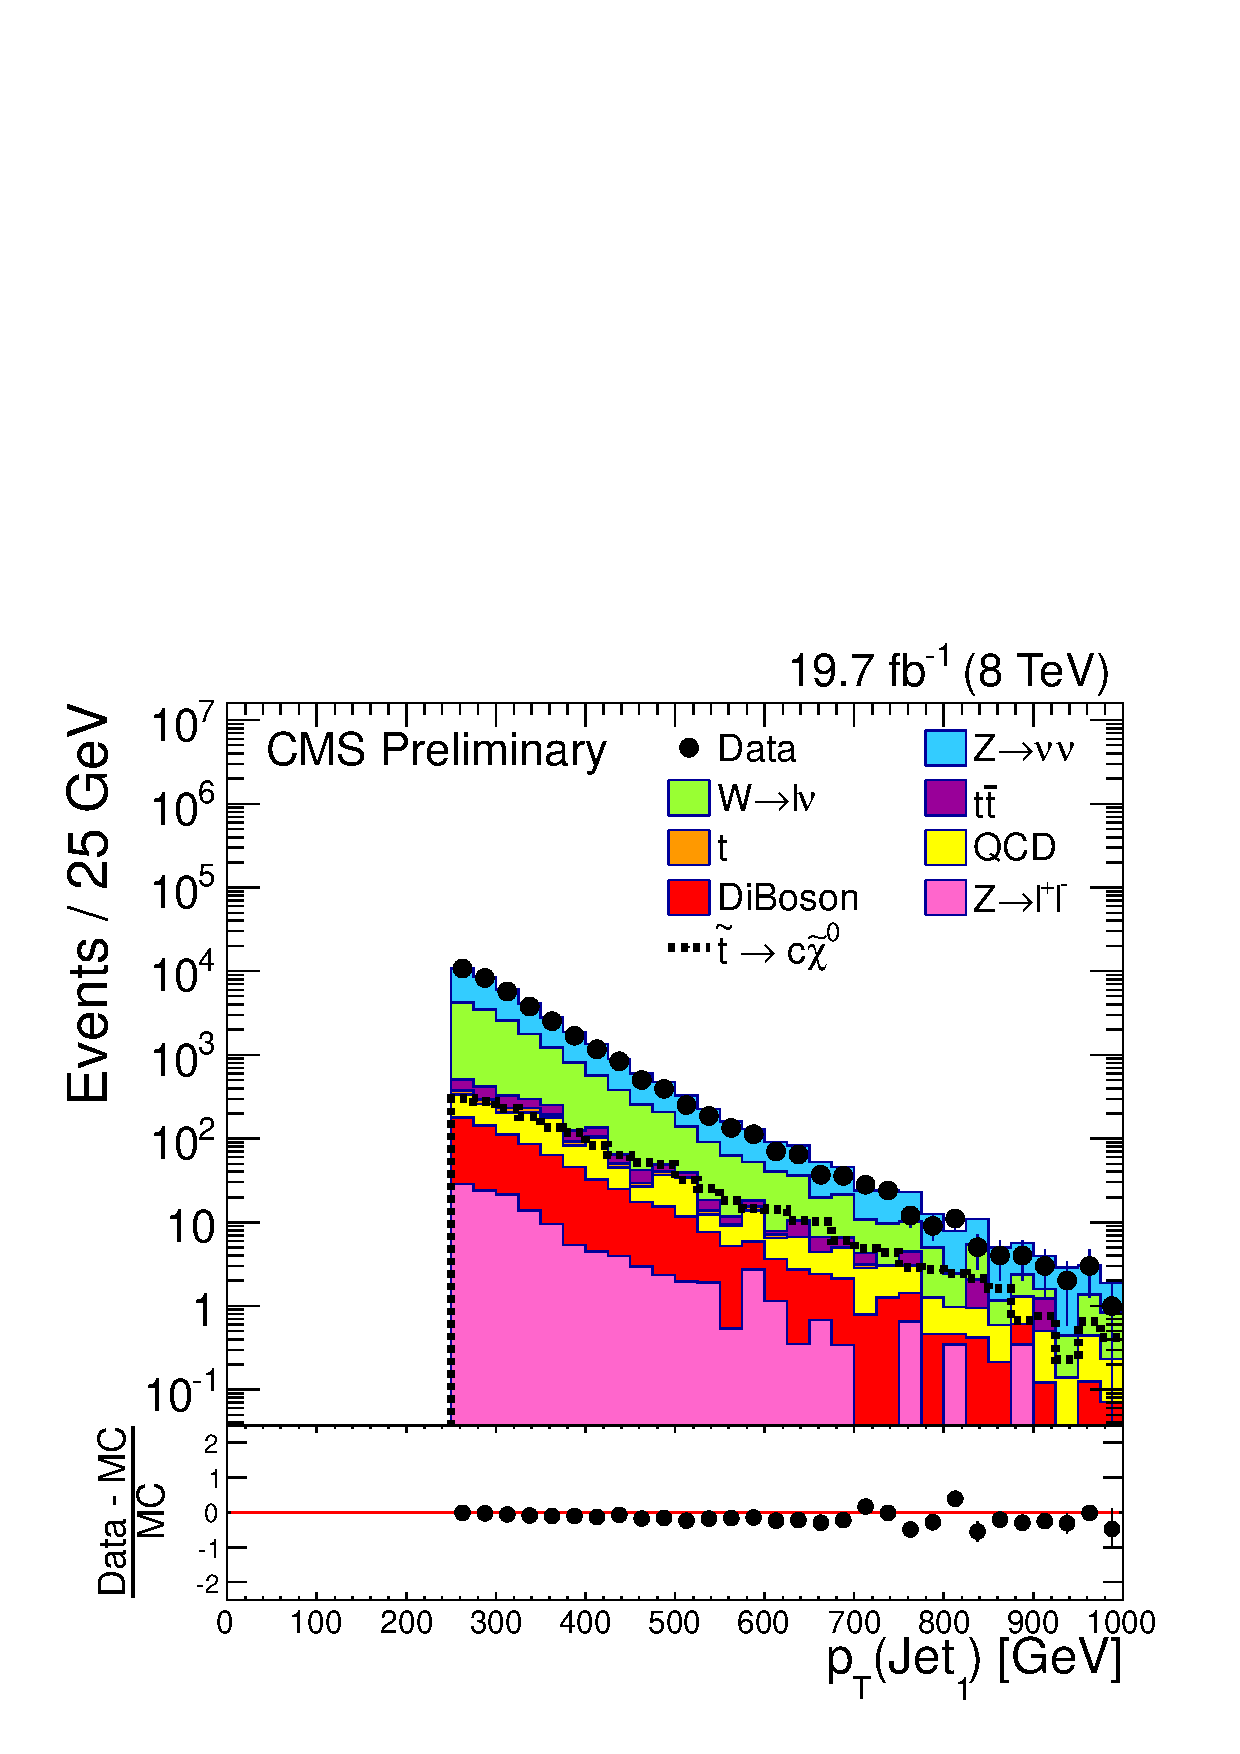
\includegraphics[scale=0.39]{Figures/sus13009/Jet1Pt.pdf}
  \caption{Distributions of (left) \METmu and (right) leading jet $\pt$ in the baseline monojet search region, $\pt(\jet_1) > 250$~\GeV, for data and SM backgrounds. Background distributions are taken from simulation, and normalized to an integrated luminosity of 19.7~\fbinv. A representative signal distribution for $\sTop \rightarrow \mathrm{c} \chiOneZero$ is also shown (in the dotted line), where $m_{\sTop} = 250~\GeV$ and $m_{\chiOneZero} = 240~\GeV$.  Statistical uncertainties are shown for the data.
  Taken from Ref.~\cite{sus14001}.
\label{fig:ANA_MET_plots}}
  \end{center}
\end{figure}


%
\section{Interpretation} 
\label{sec:GEN}

No significant deviations from the \ac{SM} predictions are observed. 
To interpret the consistency of the observed number of events with
the background expectation in the context of compressed \ac{SUSY}, and also to
enable comparison with previous results, we set limits on the production cross section of top and bottom squarks as a function of the top and bottom squark mass and the LSP mass. 

Simulation of signal events 
$\sTop\rightarrow\charmquark\chiOneZero$ and 
$\sBot\rightarrow\bottomquark\chiOneZero$ is necessary to evaluate the sensitivity of the event selection to the \ac{SMS} models probed, and therefore the compatibility of the results in Table~\ref{tab:summary_bgd} to these signatures of new physics.

\subsection{Simulation of signal events}

Simulation of signal events is in the \ac{SMS}~\cite{bib:SMS} framework as described in Section~\ref{sec:susycolliders}. 
As the monojet event selection relies on an \ac{ISR} jet, the acceptance of signal events is low due to the additional factor of $\alpha_s$ on production cross sections - typically around 1\% of events satisfy selection requirements. 
Therefore, many events are necessary to ensure uncertainties are not dominated by statistical uncertainties. 
In addition, scans consist of many points in the ($m_{\sTop}, m_{\chiOneZero}$) and ($m_{\sBot}, m_{\chiOneZero}$) mass planes in order to give good coverage across the phase space region of interest. 
As a result, millions of events are required and the signal MC simulation samples are huge - for example, the $\sTop \rightarrow \charmquark \chiOneZero$ sample takes up diskspace of order 1~TB.
Generating these samples is then a computational challenge. 
We cannot use a vast number of computing hours, nor wait years for their production. 
So, an alternative method of MC generation has been developed, as compared to the \ac{SM} background samples detailed in Section~\ref{sec:GEN}.

Events are generated using \MADGRAPH{}5 and showered with \PYTHIA{}6.4.24 with up to 2 partons. To speed up the generation process, the CMS detector response is simulated using the CMSSW FastSim prescription~\cite{FASTSIM}. 
It gives an accurate detector response to the physics objects, but takes less than 1/100$^{\rm th}$ of the time that the full \GEANTfour detector simulation takes. 
The rate of production is therefore increased by a factor 100, allowing the large samples necessary to be generated.
The MLM matching prescription~\cite{MLMmatching}, which matches hard partons from the first stage of simulation to jets produced after hadronization, is used to avoid double counting between the matrix element calculations and parton showering.
Top and bottom squark production cross sections are taken from the LHC SUSY Cross Section Working Group~\cite{bib:SUSYxs}.

Top squark signal simulation 
contains events where pair produced top squarks decay via $\sTop\rightarrow\charmquark\chiOneZero$ with 100\% branching fraction
in the ($m_{\sTop}, m_{\sTop} - m_{\chiOneZero}$) mass plane from $m_{\sTop} =$100~\GeV to 350~\GeV in steps of 25~\GeV, and 
$\dmstop = m_{\sTop} - m_{\chiOneZero} = $ 10, 20, 30, 40, 60, and 80~\GeV. 
There are two additional points at  $m_{\sTop} =$250, 275~\GeV and $\dmstop = $ 5 to probe the monojet limit towards top squark-LSP degeneracy.
An additional set of events at $m_{\sTop} =$ 200~\GeV and $m_{\sTop} - m_{\chiOneZero} =$ 10, 80~\GeV were showered with up to 3 partons.



Bottom squark signal simulation 
contains events where pair produced bottom squarks decay via $\sBot\rightarrow\bottomquark\chiOneZero$ with 100\% branching fraction
in the ($m_{\sBot}, m_{\chiOneZero}$) mass plane.
The scan is less granular, and covers a wider phase space range: 
$m_{\sBot} =$100~\GeV to 450~\GeV in steps of 25~\GeV, and 
$m_{\chiOneZero} = $ 1, 50, 100...~\GeV, for $m_{\chiOneZero} < m_{\sBot}$.
There are also points generated close to the degeneracy line, at 
$\dmsbot = m_{\sBot} - m_{\chiOneZero} = 10$~\GeV.


\section{Signal acceptance}

Here, we refer to signal acceptance as the kinetic acceptance of the signal multiplied by the efficiency of reconstruction. 

The signal acceptance in the search regions is calculated for each mass point. 
Results for the \sTop signal are shown in Figure~\ref{fig:stopAcc}, for a selection of representative values of $m_{\sTop}$.
As expected, those signal points which have the smallest mass difference \dmstop have the greatest signal acceptances, as these look most like a true monojet event. 
Signal acceptance also increases with $m_{\sTop}$.
Here, the mass difference $\dmstop$ never exceeds 80~\GeV.


\begin{figure}[ht!]
  \begin{center}
  \includegraphics[scale=0.35]{Figures/sus13009/limitplots/plots/stop/acceptance_100.pdf}
  \includegraphics[scale=0.35]{Figures/sus13009/limitplots/plots/stop/acceptance_150.pdf}
  \includegraphics[scale=0.35]{Figures/sus13009/limitplots/plots/stop/acceptance_200.pdf} 
  \includegraphics[scale=0.35]{Figures/sus13009/limitplots/plots/stop/acceptance_250.pdf}
  \includegraphics[scale=0.35]{Figures/sus13009/limitplots/plots/stop/acceptance_300.pdf} 
  \includegraphics[scale=0.35]{Figures/sus13009/limitplots/plots/stop/acceptance_350.pdf}   
   
  \caption{Signal acceptances in the search regions, at each $\pt(\jet_1)$ threshold for the process \ttwocc. Each plot shows a different value of $m_{\sTop}$, and various masses of the LSP, $m_{\chiOneZero}$. Signal acceptance is greatest when $m_{\sTop}$ is close to $m_{\chiOneZero}$, and increases with increasing $m_{\sTop}$.
\label{fig:stopAcc}}
  \end{center}
\end{figure}


The signal acceptance in the search regions for the \sBot signal are shown in Figure~\ref{fig:sbottomAcc}.
For the compressed regions, where $\dmsbot\leq100~\GeV$, we observe a similar behaviour to that seen in Figure~\ref{fig:stopAcc}.
The lower granularity of this signal compared to the \ttwocc signal is evident as there are less values of $m_{\chiOneZero}$ for each $m_{\sBot}$ in the compressed regions. 
There are also signal points for $\dmsbot > 80~\GeV$, and for low values of $m_{\chiOneZero}$, we observe relatively high signal acceptances for the lower jet threshold search regions, which then decreases at higher thresholds.
Lower numbers of events in the simulation for the mass points for which $\dmsbot\geq 150~\GeV$ is apparent, as the acceptance varies more with increasing $\pt(\jet_1)$.


\begin{figure}[ht!]
  \begin{center}
  \includegraphics[scale=0.35]{Figures/sus13009/limitplots/plots/sbottom/acceptance_100.pdf}
  \includegraphics[scale=0.35]{Figures/sus13009/limitplots/plots/sbottom/acceptance_150.pdf}
  \includegraphics[scale=0.35]{Figures/sus13009/limitplots/plots/sbottom/acceptance_250.pdf}
  \includegraphics[scale=0.35]{Figures/sus13009/limitplots/plots/sbottom/acceptance_300.pdf} 
  \includegraphics[scale=0.35]{Figures/sus13009/limitplots/plots/sbottom/acceptance_350.pdf} 
  \includegraphics[scale=0.35]{Figures/sus13009/limitplots/plots/sbottom/acceptance_400.pdf}     
  \caption{Signal acceptances in the search regions, at each $\pt(\jet_1)$ threshold for the process \ttwobb. Each plot shows a different value of $m_{\sBot}$, and various masses of the LSP, $m_{\chiOneZero}$. Signal acceptance is greatest when $m_{\sBot}$ is close to $m_{\chiOneZero}$, and increases with increasing $m_{\sTop}$.
\label{fig:sbottomAcc}}
  \end{center}
\end{figure}


Signal acceptances of some representative mass hypothesis for \ttwocc and \ttwobb signals are shown in Table~\ref{tab:mono_sigAcc} along with their statistical uncertainties. 



\newsavebox{\Boxa}
\begin{table}[h]
\small
      %  \fontsize{10 pt}{1.2 em}
        \begin{center}
        \caption{\label{tab:mono_sigAcc} Signal acceptance $\times$ efficiency, shown in \%, for each step of the event selection. 
        Two representative mass points are shown; ($m_{\sBot}$, $m_{\chiOneZero}$) = (250,240) and (150,50)~\GeV for $\ttwobb$ where $\mathcal{B}(\sBot\rightarrow\bottomquark\chiOneZero)$ = 1.0, 
        and ($m_{\sTop}$, $m_{\chiOneZero}$) = (250,240)~\GeV and (200,120) for $\ttwocc$, where $\mathcal{B}(\sTop\rightarrow\charmquark\chiOneZero)$ = 1.0.
        Only statistical uncertainties are shown.}
         \begin{lrbox}{\Boxa}
        \begin{tabular}{|l||c|c||c|c|} 
        \hline

\multirow{3}{*}{Monojet event selection } & \multicolumn{2}{c||}{$\ttwobb$} & \multicolumn{2}{c|}{$\ttwocc$} \\[0.5ex] \cline{2-5}
 & \multicolumn{2}{c||}{ $\mathcal{B}(\sBot\rightarrow\bottomquark\chiOneZero)$ = 1.0 } & \multicolumn{2}{c|}{ $\mathcal{B}(\sTop\rightarrow\charmquark\chiOneZero)$ = 1.0 }\\[0.5ex]\cline{2-5} 

 %&\multicolumn{2}{c}{  $\ttwobb$ ; $\mathcal{B}(\sbottom\rightarrow\bottomquark\chiOneZero) = 1.0$ } &\multicolumn{2}{c}{  $\ttwocc$ ; $\mathcal{B}(\sTop\rightarrow\rm{c}\chiOneZero) = 1.0$ } \\ [0.5ex]\hline

 & (250, 240)~\GeV & (150, 50)~\GeV& (250, 240)~\GeV & (200, 120)~\GeV   \\ [0.5ex]\hline

Event cleaning                     &   98.61 $\pm$   0.24 &   98.79 $\pm$  0.02 &   97.54 $\pm$   0.14  &   99.21 $\pm$  0.03 \\  
$\MET >$~200~\GeV               &   7.41 $\pm$   0.49  &   2.37 $\pm$  0.02  &    7.17 $\pm$   0.25  &    4.29 $\pm$  0.06 \\  
Noisy events                    &   6.90 $\pm$   0.47  &   2.22 $\pm$  0.02  &    6.68 $\pm$   0.24  &    4.01 $\pm$  0.06 \\  
$\pt(\jet_1)>110$~\GeV          &   6.58 $\pm$   0.46  &   2.08 $\pm$  0.02  &    6.35 $\pm$   0.23  &    3.71 $\pm$  0.06 \\  
$\njets<3$                     &   5.78 $\pm$   0.44  &   1.39 $\pm$  0.02  &    5.56 $\pm$   0.22  &    2.30 $\pm$  0.04 \\  
$\Delta \phi(\jet_1,\jet_2)<2.5$&   5.58 $\pm$   0.43  &   1.170 $\pm$  0.015  &    5.36 $\pm$   0.21  &    1.96 $\pm$  0.04 \\  
$\mu$ veto                      &   5.57 $\pm$   0.43  &   1.170 $\pm$  0.015  &    5.36 $\pm$   0.21  &    1.96 $\pm$  0.04 \\  
$\e$ veto                        &   5.57 $\pm$   0.43  &   1.160 $\pm$  0.015  &    5.36 $\pm$   0.21  &    1.96 $\pm$  0.04 \\  
$\tauh$ veto                 &   5.52 $\pm$   0.43  &   1.14 $\pm$  0.015  &    5.30 $\pm$   0.21  &    1.93 $\pm$  0.04 \\
\hline  
\MET \& $\pt(\jet_1) > 250$~\GeV&   2.08 $\pm$   0.27  &  0.222 $\pm$ 0.006  &    2.04 $\pm$   0.13  &    0.42 $\pm$  0.02 \\  
$\pt(\jet_1) > 300$~\GeV        &   1.32 $\pm$   0.21  &  0.122 $\pm$ 0.005  &    1.32 $\pm$   0.11  &    0.25 $\pm$  0.01 \\  
$\pt(\jet_1) > 350$~\GeV        &   0.80 $\pm$   0.17  &  0.058 $\pm$ 0.003  &    0.81 $\pm$  0.08  &    0.13 $\pm$  0.01 \\  
$\pt(\jet_1) > 400$~\GeV        &   0.49 $\pm$   0.13  &  0.027 $\pm$ 0.002  &    0.50 $\pm$  0.07  &   0.072 $\pm$ 0.008 \\  
$\pt(\jet_1) > 450$~\GeV        &   0.31 $\pm$   0.11  &  0.016 $\pm$ 0.002  &    0.32 $\pm$  0.05  &   0.041 $\pm$ 0.006 \\  
$\pt(\jet_1) > 500$~\GeV        &   0.19 $\pm$  0.08  &  0.009 $\pm$ 0.001  &    0.19 $\pm$  0.04  &   0.023 $\pm$ 0.005 \\  
$\pt(\jet_1) > 550$~\GeV        &   0.12 $\pm$  0.07  &  0.006 $\pm$ 0.001  &    0.12 $\pm$  0.03  &   0.013 $\pm$ 0.003 \\ \hline
\end{tabular}
\end{lrbox}
\scalebox{0.90}{\usebox{\Boxa}}
\end{center}
\end{table}
 




\subsection{Signal acceptance in 2- and 3-parton simulation}

The difference in signal acceptance between the 2-parton and 3-parton samples produced for \ttwocc 
is found to be small; Table~\ref{tab:2_3_partonAcc} lists the acceptances for both samples.
In the signal regions the differences in the acceptance is, at most, 0.04\%, 
and generally it is less where the analysis is most sensitive (for small mass differences).
We conclude the effect of generating 2 or 3 partons with the signal does not have a significant effect on the result.
Nevertheless, the differences are accounted for in the uncertainty on the signal acceptance.

\newsavebox{\Boxb}
\begin{table}[!Hhtb]
\begin{center}
\caption{Acceptances (in \%) of 2-parton and 3-parton samples for mass points ($m_{\sTop}, m_{\chiOneZero}$) = (200,190)~\GeV and (200,120)~\GeV. The modulus of the differences in the acceptances from the two samples are listed. } 
\label{tab:2_3_partonAcc}
\begin{lrbox}{\Boxb}
\begin{tabular}{ l |ccc|ccc} \hline
 \multicolumn{1}{c|}{\multirow{2}{*}{ Event selection}} & \multicolumn{3}{c|}{($m_{\sTop}, m_{\chiOneZero}$) = (200,190)}& \multicolumn{3}{c}{($m_{\sTop}, m_{\chiOneZero}$) = (200,120)} \\ 
    &  2 partons  & 3 partons & $|$Difference$|$ &  2 partons & 3 partons & $|$Difference$|$\\ 
    \hline
Abnormal events         & 97.1  & 97.1  & 0     & 99.3  & 99.19 & 0.11  \\
$\METmu > 200~\GeV$     & 2.74  & 2.61  & 0.13  & 1.84  & 1.79  & 0.05  \\
Noise clean             & 2.58  & 2.47  & 0.11  & 1.75  & 1.71  & 0.04  \\
$\pt(\jet_1)>110~\GeV$  & 12.53 & 2.42  & 0.11  & 1.71  & 1.68  & 0.03  \\
$\njets<3$              & 2.14  & 2.06  & 0.08  & 0.94  & 0.98  & 0.04  \\
$\Delta \phi(\jet_1, \jet_2) <2.5$ &2.05  & 1.99  & 0.06  & 0.78  & 0.79  &  0.01 \\
$\e$ veto               & 2.05  & 1.99  & 0.06  & 0.78  & 0.79  &  0.01 \\
$\mu$ veto              & 2.05  & 1.99  & 0.06  & 0.78  & 0.79  &  0.01 \\
$\tauh$ veto            & 2.02  & 1.97  & 0.05  & 0.77  & 0.77  & 0     \\
$\pt(\,\mathrm{j}_1)>250$~\GeV & \multirow{2}{*}{1.32}
       & \multirow{2}{*}{1.36}   
       & \multirow{2}{*}{0.04}
       & \multirow{2}{*}{0.43}
       & \multirow{2}{*}{0.41}
       & \multirow{2}{*}{0.02}\\
               \,\,\& $\METmu>250$~\GeV   &   &   &   &   &               \\
$\pt(\jet_1)$$>$300~\GeV  & 0.86  & 0.88  &  0.02 & 0.25  & 0.23  & 0.02  \\
$\pt(\jet_1)$$>$350~\GeV  & 0.51  & 0.51  & 0     & 0.14  & 0.12  & 0.02  \\
$\pt(\jet_1)$$>$400~\GeV  & 0.30  & 0.30  & 0     & 0.076 & 0.063 & 0.013 \\
$\pt(\jet_1)$$>$450~\GeV  & 0.17  & 0.18  &  0.01 & 0.042 & 0.025 & 0.017 \\
$\pt(\jet_1)$$>$500~\GeV  & 0.10  & 0.10  & 0     & 0.024 & 0.013 & 0.011 \\
$\pt(\jet_1)$$>$550~\GeV  & 0.067 & 0.056 & 0.011 & 0.014 & 0.006 & 0.008 \\
\hline
\end{tabular}  
\end{lrbox}
\scalebox{0.87}{\usebox{\Boxb}}    
\end{center}
\end{table}


\subsection{Systematic Uncertainties on Signal}
\label{sec:signalSYST}

% The analysis is reliant upon an \ac{ISR} jet, thus the signal modelling of \ac{ISR} is very important.
% This is the dominant source of uncertainty on the signal.

The selection of signal events (and therefore the signal acceptance) in this analysis relies on a high-\pt ISR jet, so the modelling of ISR must be reliable.
The simulated and measured \pt spectra of recoiling systems against ISR jets is studied in Ref.~\cite{CMSsinglelep} for Z\,+\,jets, 
\ttbar and other processes. 
The simulation is found to over predict the data by 20\% for ISR jets with $\pt > 250$ \GeV, see Figure~\ref{fig:ISRsyst}.
All signal acceptances have therefore been weighted by a factor of 0.8 to correct for this difference, and a systematic uncertainty of 20\% is assigned to each search region to account for this difference for the high \pt ISR jets involved.

\begin{figure}[ht!]
  \begin{center}
  \includegraphics[scale=0.35]{Figures/sus13009/ISRmodellingSUS13011.pdf}
  \caption{Taken from~\cite{CMSsinglelep}, the comparison of data to the prediction from simulation of the jet recoil system in \ttbar events. The data/MC ratio, in the top of the figure, shows that for jets $>250~\GeV$, the simulation over predicts the data.
\label{fig:ISRsyst}}
  \end{center}
\end{figure}


Other sources of uncertainty on the signal are considered. They are:
\begin{itemize}
  \item the uncertainty on the \ac{JES}, which is evaluated by taking the difference in acceptances when the jet \ptv is shifted up and down by an $\eta$ and $\pt$ dependent factor. The difference in acceptances between varying the energy scale up and down is less than 1\% in the signal regions: see Table~\ref{tab:JESuncert}. 
  \item uncertainties on the \ac{PDFs}. The PDF uncertainty for a representative signal sample was found to be less than 2$\%$. 
  \item the difference in acceptance that is obtained from generating signal events with up to 3 partons in \MADGRAPH rather than 2 partons ($<1\%$). 
\end{itemize}

The total uncertainty on the signal in each signal region is taken to be a conservative 25$\%$.
The error on the luminosity measurement is 2.6\% ~\cite{lumi:Summer2013}.

\newsavebox{\Boxc}
\begin{table}[!Hhtb]
\begin{center}
\caption{Acceptances (in \%) of signal samples for mass points ($m_{\sTop}, m_{\chiOneZero}$) = (200,190)~\GeV and (200,120)~\GeV, for when the energy scale is increased and decreased. The modulus of the differences in the acceptances from the two samples are listed. } 
\label{tab:JESuncert}
\begin{lrbox}{\Boxc}
\begin{tabular}{ l |ccc|ccc} \hline
 \multicolumn{1}{c|}{\multirow{2}{*}{ Search region}} & \multicolumn{3}{c|}{($m_{\sTop}, m_{\chiOneZero}$) = (200,190)}& \multicolumn{3}{c}{($m_{\sTop}, m_{\chiOneZero}$) = (200,120)} \\ 
    & JES +  & JES - & $|$Difference$|$ &  JES + & JES - & $|$Difference$|$\\ 
   \hline
$\pt(\jet_1)$$>$300~\GeV & 1.33 & 1.33 & $<$0.01 & 0.42 & 0.44 & 0.03    \\
$\pt(\jet_1)$$>$300~\GeV & 0.88 & 0.84 & 0.03    & 0.26 & 0.26 & $<$0.01  \\
$\pt(\jet_1)$$>$300~\GeV & 0.52 & 0.50 & 0.03    & 0.14 & 0.14 & $<$0.01   \\
$\pt(\jet_1)$$>$300~\GeV & 0.30 & 0.29 & 0.01    & 0.07 & 0.08 & $<$0.01  \\
$\pt(\jet_1)$$>$300~\GeV & 0.18 & 0.17 & 0.01    & 0.04 & 0.04 & $<$0.01       \\
$\pt(\jet_1)$$>$300~\GeV & 0.11 & 0.10 & 0.01    & 0.02 & 0.02 & $<$0.01   \\
$\pt(\jet_1)$$>$300~\GeV & 0.07 & 0.06 & $<$0.01 & 0.02 & 0.01 & $<$0.01   \\
\hline
\end{tabular}  
\end{lrbox}
\scalebox{0.97}{\usebox{\Boxc}}    
\end{center}
\end{table}



\section{Exclusion limits}
\label{sec:STAT}

The CL$_{s}$ method is used to estimate the 95\% confidence level (CL) for a signal cross section in a counting experiment~\cite{bib:STAT_RooStats,PDG}.
Given the integrated luminosity, signal acceptance, background expectation and number of observed events (with associated uncertainties),
the 95\% CL upper limit on the signal cross section is calculated.
The theoretical top-squark production cross sections, which are equal to the bottom-squark production cross sections, and $\pm1\sigma_{\rm th}$ bands are taken from a collaboration between the \ac{ATLAS}, \ac{CMS}
and \ac{LPCC} \ac{SUSY} working groups. Theory uncertainties are dominated by PDF uncertainties 
and calculations are detailed in Ref.~\cite{bib:SUSYxs}. 
Cross section values can be found in Ref.~\cite{stopsbottomxs}.  
The 95\% CL exclusion limits on production cross sections are compared to the theoretical expectations in order to set lower limits on the top (bottom) squark and LSP masses in the $m_{\sTop}, m_{\chiOneZero}$ ($m_{\sBot}, m_{\chiOneZero}$) mass plane. 


\begin{figure}[!Ht]
  \begin{center}
  \includegraphics[scale=0.35]{Figures/sus13009/limitplots/plots/stop/expected_100.pdf}
  \includegraphics[scale=0.35]{Figures/sus13009/limitplots/plots/stop/expected_150.pdf}
  \includegraphics[scale=0.35]{Figures/sus13009/limitplots/plots/stop/expected_200.pdf} 
  \includegraphics[scale=0.35]{Figures/sus13009/limitplots/plots/stop/expected_250.pdf}
  \includegraphics[scale=0.35]{Figures/sus13009/limitplots/plots/stop/expected_300.pdf} 
  \includegraphics[scale=0.35]{Figures/sus13009/limitplots/plots/stop/expected_350.pdf}  
  \caption{95\% CL expected limit on top-squark production cross section as a function of $\pt(j_{1})$\GeV (i.e. in each search region). Limits for $m_{\sTop}=100,150,200,250,300$ and 350~\GeV are shown, where each line corresponds to $\dmstop=10,20,30,40,60$ and 80~\GeV.}
  \label{fig:expLimStop}
  \end{center}
\end{figure}

Expected limits, displayed as a function of $\pt(\,\mathrm{j}_1)$ for every signal mass hypothesis for the \ttwocc signal, using the background expectation in each search region,
can be found in Figure~\ref{fig:expLimStop} where each plot shows a particular $m_{\sTop}$. 
Similar plots showing the 95\% CL expected limits for the \ttwobb signal are shown in 
Figure~\ref{fig:expLimSbot}.
The signal region where the best (i.e. lowest) expected limit is found is selected as the optimal region in which to set limits for that mass point.
Limits are generally fairly flat across the phase space range, for those mass points in the compressed region where \dmstop and $\dmsbot \lessapprox 100~\GeV$.
A fluctuation in the number of $Z(\mu\mu)$ events at $\pt(\,\mathrm{j}_1)>450$~\GeV leads to a fluctuation in the total background expectation in this search region. 
To ensure smooth limit curves we have discounted this signal region from the limit setting procedure.
For the curves shown in Figure~\ref{fig:expLimSbot}, we are not able to set a limit on the production section of bottom squarks for some mass points when \dmsbot is large (i.e. not the compressed SUSY models) in the search regions with the highest $\pt(\jet_1)$ thresholds. 
This is because the analysis looses sensitivity due to hard cuts on ISR combined with the jet multiplicity requirements.


\begin{figure}[!Hhtb]
  \begin{center}
  \includegraphics[scale=0.35]{Figures/sus13009/limitplots/plots/sbottom/expected_100.pdf}
  \includegraphics[scale=0.35]{Figures/sus13009/limitplots/plots/sbottom/expected_150.pdf}
  \includegraphics[scale=0.35]{Figures/sus13009/limitplots/plots/sbottom/expected_200.pdf} 
  \includegraphics[scale=0.35]{Figures/sus13009/limitplots/plots/sbottom/expected_250.pdf}
  \includegraphics[scale=0.35]{Figures/sus13009/limitplots/plots/sbottom/expected_300.pdf} 
  \includegraphics[scale=0.35]{Figures/sus13009/limitplots/plots/sbottom/expected_350.pdf} 
  \caption{95\% CL expected limit on bottom-squark production cross section as a function of $\pt(j_{1})$\GeV (i.e. in each search region). Limits for $m_{\sBot}=100,150,200,250,300$ and 350~\GeV are shown, where each line corresponds to a different $m_{\chiOneZero}$.}
  \label{fig:expLimSbot}
  \end{center}
\end{figure}


The temperature plots in Figure~\ref{fig:optimalacc} show the signal acceptance in the search region with the best expected limit for both ($m_{\sTop}, m_{\chiOneZero}$) and ($m_{\sBot}, m_{\chiOneZero}$) mass planes.
The temperature plots in Figure~\ref{fig:optimalExp} show the best expected 95\% CL limit across the phase space range, and Figure~\ref{fig:optimalJ1} shows the search region in which this best expected limit is found.
We see that typically, harder leading jet cuts give the better limits along the diagonal, where events are dominated by ISR. 
Also, for larger $m_{\sTop}$ and $m_{\sBot}$, harder jet thresholds give the better limits, as these events are typically more boosted.   


\begin{figure}[!Hhtb]
  \begin{center}
  \includegraphics[scale=0.39]{Figures/sus13009/limitplots/plots/stop/optimal_stop_acceptance.pdf}
  \includegraphics[scale=0.39]{Figures/sus13009/limitplots/plots/sbottom/optimal_sbottom_acceptance.pdf}
  \caption{The temperature plot shows acceptance of the signal point where the best expected limit is found, across the ($m_{\sTop}, m_{\chiOneZero})$ (left) and ($m_{\sBot},m_{\chiOneZero}$) (right) mass planes.}
  \label{fig:optimalacc}
  \end{center}
\end{figure}

\begin{figure}[!Hhtb]
  \begin{center}
  \includegraphics[scale=0.39]{Figures/sus13009/limitplots/plots/stop/optimal_stop_expected.pdf}
  \includegraphics[scale=0.39]{Figures/sus13009/limitplots/plots/sbottom/optimal_sbottom_expected.pdf}
  \caption{The temperature plot shows the best expected limit across the ($m_{\sTop}, m_{\chiOneZero})$ (left) and ($m_{\sBot},m_{\chiOneZero}$) (right) mass planes.}
  \label{fig:optimalExp}
  \end{center}
\end{figure}

\begin{figure}[!Hhtb]
  \begin{center}
  \includegraphics[scale=0.39]{Figures/sus13009/limitplots/optimal_stop_jet1pT.pdf}
  \includegraphics[scale=0.39]{Figures/sus13009/limitplots/optimal_sbottom_jet1pT.pdf}
  \caption{The temperature plot shows search region (the $\pt(\,\mathrm{j}_1)$ threshold) in which the best expected limit is found, across the ($m_{\sTop}, m_{\chiOneZero})$ (left) and ($m_{\sBot},m_{\chiOneZero}$) (right) mass planes. Plots feature in Ref.~\cite{sus14001}.}
  \label{fig:optimalJ1}
  \end{center}
\end{figure}

In the ($m_{\sBot}, m_{\chiOneZero}$) mass plane we also expect sensitivity outside of the compressed region. 
The bottom squark decay $\sBot \rightarrow \bottomquark \chiOneZero$ is valid for mass points that lie outside of similar region in which the top squark decay $\sTop \rightarrow \charmquark \chiOneZero$ dominates, so we are also able to test the sensitivity of the search criteria for signals where $\dmsbot>m_{\W}$.
To understand the signal acceptances outside of the region, we study several mass points for which $m_{\sBot}=225~\GeV$. 
Figure~\ref{fig:sbot225njets} shows the jet multiplicity distributions for $m_{\chiOneZero}=1,50$ and 100~\GeV in the baseline search region where all criteria apart from $\njets<2$ have been applied.  

\begin{figure}[!Hhtb]
  \begin{center}
  \includegraphics[scale=0.39]{Figures/sus13009/Njets_225_Norm.pdf}
  \caption{Normalized distribution of \njets for $\sBot \rightarrow \bottomquark \chiOneZero$ signal points, in the events satisfying the baseline search region criteria, other than $\njets<3$. Signal points are labelled as ($m_{\sBot}, m_{\chiOneZero}$)~\GeV.}
  \label{fig:sbot225njets}
  \end{center}
\end{figure}

%reasons for b-jet limit
As $m_{\chiOneZero}$ decreases, there are fewer events with \njets=1, and more events with higher jet multiplicities. 
This is to be expected, as decay products become harder and a final state single high-\pt jet originating from \ac{ISR} is no longer seen. 
At ($m_{\sBot},m_{\chiOneZero}$) = (225, 100)~\GeV, most events contain one jet. This could be an ISR jet, or similarly a b-jet from the decay of the bottom squark which is energetic enough to pass the $\pt(\jet_1)$ requirement of the baseline signal region.
A significant number of events contain three jets, where the most energetic jet with $\pt>250~\GeV$ is from one of the b-quark decays (or \ac{ISR}), and the two further jets with $\pt>60~\GeV$ are from the second b quark and ISR (or the two b quarks or otherwise). 
These trijet events do not satisfy the requirements of the search region and so acceptance suffers. 
As \dmsbot increases further, at ($m_{\sBot},m_{\chiOneZero}$) = (225, 50)~\GeV, we see most events are classified as having one or two jets. 
Here, the jets are mostly from b quark decay, as both are energetic enough to pass the jet criteria.
Crucially, most of these events will satisfy the search region requirements once $\njets<3$ is applied: the search regions are therefore dijet dominated.
At ($m_{\sBot},m_{\chiOneZero}$)=(225,1)~\GeV we see that more events sit at the higher jet multiplicities. 
We are less dominated by energetic jets from ISR here; instead the \dmsbot is now large enough that b quarks get a significant boost and satisfy $\pt(\jet_1)>250~\GeV$, $\pt(\jet_2)>60~\GeV$. There are more events with softer ISR or FSR jets which push the jet multiplicity up, and reduce the signal acceptance.

Outside of the compressed region, we are then not dominated by \ac{ISR} jets. Optimal signal regions are therefore typically those lower $\pt(\jet_1)$ thresholds, as seen in Figure~\ref{fig:optimalJ1}.
Figure~\ref{fig:jetContent225} shows the origin of jets for the same mass points for events that satisfy the baseline search criteria, including the $\njets<3$ requirement.
The behaviours described above are evident. 

\begin{figure}[!Hhtb]
  \begin{center}
  \includegraphics[scale=0.39]{Figures/sus13009/eventTypes_225.pdf}
  \caption{The topology of events satisfying the baseline search region criteria for ($m_{\sBot}, m_{\chiOneZero}$)=(225,1), (225,50) and (225,100)~\GeV. The origin of the first and second jet in the event is shown for events with one or two jets. Distributions are normalized to unit area.}
  \label{fig:jetContent225}
  \end{center}
\end{figure}

%
Figure~\ref{fig:stop_limits} shows the best 95\% CL expected and observed limits on the top-squark production cross section, 
as a function of the top squark mass for $\dmstop = 10, 20, 30, 40, 60$ and $80~\GeV$.
Figure~\ref{fig:sbottom_10GeV} shows the similar 95\% CL expected and observed limits on the bottom-squark production cross section, 
as a function of the bottom squark mass for $\dmstop = 10$. 
As mass points in the remainder of the bottom squark signal sample are produced in a regular pattern in $(m_{\sBot}, m_{\chiOneZero})$ rather than in $(m_{\sBot}, \dmsbot)$ (as in the \ttwocc case), we show the results for the remainder of $\ttwobb$ phase space in a slightly different plane.
Figure~\ref{fig:sbottom_limits} shows the best expected and observed limits for various bottom squark masses as a function of mass difference, $\dmsbot$.
All plots also show the $\pm1,2 \sigma_{\rm exp}$ bands on the expected limits.




%The results of the monojet search can also be interpreted to constrain the production of light stops. The observed limits on the production cross section as a function of the stop mass are shown in Figure~\ref{fig:stop_limits} for mass splittings of 10 GeV, 30 GeV and 80 GeV. Also shown are the expected limits and the theoretical prediction. The observed (expected) limits on the stop mass for the 10 GeV and 30 GeV mass splitting are; 250 (255) GeV and 190 (195) GeV respectively.
\begin{figure}[!Hhtb]
  \begin{center}
%  \includegraphics[scale=0.39]{m10.pdf}
%  \includegraphics[scale=0.39]{m30.pdf}
%  \includegraphics[scale=0.39]{Figures/sus13009/limitplots/plots/stop/Limit_susy_stop_10.pdf}
%  \includegraphics[scale=0.39]{Figures/sus13009/limitplots/plots/stop/Limit_susy_stop_20.pdf}
%  \includegraphics[scale=0.39]{Figures/sus13009/limitplots/plots/stop/Limit_susy_stop_30.pdf}
%  \includegraphics[scale=0.39]{Figures/sus13009/limitplots/plots/stop/Limit_susy_stop_40.pdf}
%  \includegraphics[scale=0.39]{Figures/sus13009/limitplots/plots/stop/Limit_susy_stop_60.pdf}
%  \includegraphics[scale=0.39]{Figures/sus13009/limitplots/plots/stop/Limit_susy_stop_80.pdf}
  \includegraphics[scale=0.39]{Figures/sus13009/limits//Limit10.pdf}
  \includegraphics[scale=0.39]{Figures/sus13009/limits//Limit20.pdf}
  \includegraphics[scale=0.39]{Figures/sus13009/limits//Limit30.pdf}
  \includegraphics[scale=0.39]{Figures/sus13009/limits//Limit40.pdf}
  \includegraphics[scale=0.39]{Figures/sus13009/limits//Limit60.pdf}
  \includegraphics[scale=0.39]{Figures/sus13009/limits//Limit80.pdf}
  \caption{95\% CL observed and expected limits on the top-squark production cross section as a function of the $m_{\sTop}$ for $m_{\sTop} - m_{\chiOneZero} = 10, 20, 30, 40, 60$ and 80 \GeV. Curves taken from Ref.~\cite{sus13009}.}
  \label{fig:stop_limits}
  \end{center}
\end{figure}

The observed behaviour in Figure~\ref{fig:sbottom_limits} where sbottom quark limits are low for the compressed region, at low $\dmsbot$, increase, and then decrease again for larger \dmsbot is due to the migration of events between bins in jet multiplicity, as described above. 
The signal topology and search region jet requirements means monojet events, dijet events, and higher jet multiplicities dominate in the different regions of phase space and signal acceptance (and hence limits) respond accordingly. 

 % The limits at low mass difference are due to monojet events, 
 %  where an event with a radiated ISR jet passes the event selection. 
 %  At large mass differences, we become sensitive to dijet events; events in which two b-jets from both bottom squark decays pass the event selection.

\begin{figure}[!Hhtb]
  \begin{center}
%  \includegraphics[scale=0.39]{m10.pdf}
%  \includegraphics[scale=0.39]{m30.pdf}
  \includegraphics[scale=0.39]{Figures/sus13009/limitplots/plots/sbottom/Limit_susy_sbottom_10.pdf}
  \caption{95\% CL observed and expected limits on the bottom-squark production cross section as a function of $m_{\sBot}$ for $m_{\sBot} - m_{\chiOneZero} = 10~\GeV$.}
  \label{fig:sbottom_10GeV}
  \end{center}
\end{figure}

\begin{figure}[!Hhtb]
  \begin{center}
  \includegraphics[scale=0.39]{Figures/sus13009/limitplots/plots/sbottom/Limit_DM_sbottom_100.pdf}
  \includegraphics[scale=0.39]{Figures/sus13009/limitplots/plots/sbottom/Limit_DM_sbottom_150.pdf}
  \includegraphics[scale=0.39]{Figures/sus13009/limitplots/plots/sbottom/Limit_DM_sbottom_175.pdf}
  \includegraphics[scale=0.39]{Figures/sus13009/limitplots/plots/sbottom/Limit_DM_sbottom_200.pdf}
  \includegraphics[scale=0.39]{Figures/sus13009/limitplots/plots/sbottom/Limit_DM_sbottom_225.pdf}
  \includegraphics[scale=0.39]{Figures/sus13009/limitplots/plots/sbottom/Limit_DM_sbottom_250.pdf}
  \includegraphics[scale=0.39]{Figures/sus13009/limitplots/plots/sbottom/Limit_DM_sbottom_275.pdf}
    \includegraphics[scale=0.39]{Figures/sus13009/limitplots/plots/sbottom/Limit_DM_sbottom_300.pdf}
  \caption{95\% CL observed and expected limits on the bottom-squark production cross section as a function of the mass difference $m_{\sBot} - m_{\chiOneZero}$, shown for $m_{\sBot} = 100, 150, 175, 200, 225,$ and 275~\GeV. 
  Also shown are the $\pm 1, 2 \sigma_{\rm exp}$ limits. 
 }
  \label{fig:sbottom_limits}
  \end{center}
\end{figure}




Masses where the observed (expected) limits lie beneath the theory cross section we observe (expect) to exclude.
By finding the point of intersection between the observed (expected) and theoretical cross sections, we find the observed (expected) lower limit on the mass of the top or bottom squark for a particular value of $m_{\chiOneZero}$.
Similarly, by finding the intersection between the observed ($\pm 1 \sigma_{\rm exp}$) and $\pm 1 \sigma_{\rm th}$ (theoretical) limits on cross sections, we find the $\pm 1 \sigma_{\rm th}$ ( $\pm 1  \sigma_{\rm exp}$) lower limits on masses.
By doing this for every mass point available we build a contour in the ($m_{\sTop},m_{\chiOneZero}$) and ($m_{\sBot},m_{\chiOneZero}$) mass planes.

Figure~\ref{fig:stop_limits_2D} shows 95\% CL expected $\pm 1 \sigma_{\rm exp}$ and observed limits $\pm 1 \sigma_{\rm th}$ in the ($m_{\sTop},m_{\chiOneZero}$) mass plane assuming 100\% branching fraction to the top squark decay $\sTop \rightarrow \charmquark \chiOneZero$.
Also shown are previous results from the Tevatron.
We are able to exclude the region above a line which goes from approximately $m_{\sTop}=130~\GeV, m_{\chiOneZero}=50~\GeV$ to $m_{\sTop}=260~\GeV, m_{\chiOneZero}=255~\GeV$.  
Because the analysis is insensitive to the final state decay products, we are able to exclude \ttwocc production for $m_{\sTop} \leq 260~\GeV$ and $\dmstop \leq 10~\GeV$: right up to the degeneracy limit. 

Similarly, Figure~\ref{fig:sbottom_limits_2D} shows the 95\% CL expected $\pm 1 \sigma_{\rm exp}$ and observed limits $\pm 1 \sigma_{\rm th}$ in the ($m_{\sBot},m_{\chiOneZero}$) mass plane assuming 100\% branching fraction to bottom squark decay $\sBot \rightarrow \bottomquark \chiOneZero$.
We are able to exclude the region above a line which goes from approximately $m_{\sBot}=140~\GeV, m_{\chiOneZero}=50~\GeV$ to $m_{\sBot}=270~\GeV, m_{\chiOneZero}=265~\GeV$.  
Further, the region where $m_{\sBot} < 165~\GeV$ is excluded for all $m_{\chiOneZero}$.
We also exclude a region at lower $m_{\chiOneZero}$ from approximately $m_{\sBot}=150~\GeV, m_{\chiOneZero}=40~\GeV$ to $m_{\sBot}=275~\GeV, m_{\chiOneZero}=60~\GeV$, above the line extending from $m_{\sBot}=175~\GeV, m_{\chiOneZero}=0~\GeV$ to $m_{\sBot}=275~\GeV, m_{\chiOneZero}=40~\GeV$.
The limit in the compressed region echoes that from the ($m_{\sTop},m_{\chiOneZero}$) mass plane: monojet-like events dominate, and sensitivity to events in the region of the mass plane where decay products are very soft is achieved. 
In the region $\dmsbot>m_{\W}$, we are set limits on $m_{\sBot}$ outside the compressed region. The bottom squark decay products are much more energetic, and dijet events, where both events are both b decay, dominate. 



\begin{figure}[!Hhtb]
  \begin{center}
%  \includegraphics[scale=0.39]{m10.pdf}
%  \includegraphics[scale=0.39]{m30.pdf}
  \includegraphics[scale=0.39]{Figures/sus13009/limits/limits_stopLSP.pdf}
%  \includegraphics[scale=0.39]{Figures/sus13009/limits/limits_stopDM.pdf}
  \caption{ Expected and observed 95\% CL exclusion limits in the ($m_{\sTop}, m_{\chiOneZero}$) mass plane for top-squark pair production, assuming 100\% branching fraction to the decay $\sTop \rightarrow \charmquark \chiOneZero$. The $\pm1\sigma_{exp}$ and $\pm1\sigma_{th}$ curves are also shown. The diagonal grey lines mark the borders of the kinematic regimes surrounding the compressed region of phase space. 
  Taken from Ref.~\cite{sus13009}.}
  \label{fig:stop_limits_2D}
  \end{center}
\end{figure}


\begin{figure}[!Hhtb]
  \begin{center}
  \includegraphics[scale=0.39]{Figures/sus13009/limits/mstop_lsp.pdf}
  \includegraphics[scale=0.39]{Figures/sus13009/sbottomlimits/msbottom_lsp.pdf}
  \caption{ Observed and expected limits on top-(left) and bottom-(right) squark pair production cross section as a function of the top and bottom squark mass and LSP mass. The top squark limit is the same as the above, only formatted to allow easy comparison between the two limits, which are very similar in the compressed region, as is expected. Additional sensitivity around $m_{\sBot}\approx50~\GeV$ arises from dijet events which satisfy the search region criteria.
  These curves are those taken from Ref.~\cite{sus14001}.}
  \label{fig:sbottom_limits_2D}
  \end{center}
\end{figure}

\section{Summary}
A search has been performed for signatures of top and bottom squark production in events with a monojet and large \METmu, using an integrated luminosity of 19.7~\fbinv of pp collisions at 8~\TeV. 
The data are found to be in good agreement with expected contributions from \ac{SM} processes.  
Limits on top and bottom squark production cross sections in the context of \ac{SMS} are set. 
Comparisons with the predictions from theory allows limits on third generation squark masses to be set in a mass parameter space which is insensitive to previous searches: where mass splittings between the \sTop and \sBot squark and the LSP are less than $\approx$ 80~\GeV.  
We exclude $\ttwocc$ 
production for $m_{\sTop} \leq 260~\GeV$ and
$m_{\sTop} - m_{\chiOneZero} <10~\GeV$ 
and analogously for $m_{\sTop} \leq 120~\GeV$ and
$m_{\sTop} - m_{\chiOneZero} <80~\GeV$.
We similarly exclude $\ttwobb$ production for $m_{\sBot} \leq 270~\GeV$ and 
$(m_{\sBot} - m_{\chiOneZero}) <10~\GeV$, with all $m_{\chiOneZero}$ excluded for $m_{\sTop} \leq 145~\GeV$.
A small region of $\ttwobb$ parameter space is excluded for $m_{\sBot} \leq 270~\GeV$ and $m_{\chiOneZero} \approx 50~\GeV$.
Because the final state jets in this search are invisible, and we are independent of the final state, these limits can be generalized to $\sTop \rightarrow x \chiOneZero$ and $\sBot \rightarrow x \chiOneZero$, where $x$ is any state which is invisible within the event selection.



% \begin{table*}%[!Hhtb]  %table 8   110811:05  
%         \begin{center}  
%         \renewcommand{\arraystretch}{1.5}
% \caption{The expected limits on the production cross section of stops for different values of \dmstop. 
% Also shown are the +1$\sigma$ expected limits in superscript, and the -1$\sigma$ expected limits in subscript.}
% \label{tab:expected_limits}
% \small
%                         \begin{tabular}{l|ccccccc} \hline
% $\pt(\,\mathrm{j}_1)$ (\GeV)   &  $> 250$ &   $> 300$ &  $> 350$ &  $> 400$ &  $> 450$ &  $> 500$ &  $> 550$  \\ \hline
% \dmstop = 10~\GeV&  $ 82.98 \pm ^{ 115.7 }_{ 57.15 } $ &    $ 37.63 \pm ^{ 53.28 }_{ 28.11 } $ &    $ 23.89 \pm ^{ 33.84 }_{ 17.85 } $ &    $ 15.48 \pm ^{ 21.93 }_{ 11.56 } $ &    $ 11.02 \pm ^{ 17.5 }_{ 8.489 } $ &   $ 8.128 \pm ^{ 12.9 }_{ 6.259 } $ &   $ 6.148 \pm ^{ 9.758 }_{ 4.734 } $ \\ 
% \dmstop = 20~\GeV&   $ 129 \pm ^{ 178.2 }_{ 88.96 } $ &    $ 57.03 \pm ^{ 81.5 }_{ 39.17 } $ &   $ 32.37 \pm ^{ 46.33 }_{ 22.24 } $ &    $ 20.32 \pm ^{ 28.99 }_{ 13.96 } $ &    $ 14.1 \pm ^{ 20.16 }_{ 9.686 } $ &   $ 10.59 \pm ^{ 15.01 }_{ 7.916 } $ &    $ 7.658 \pm ^{ 12.11 }_{ 5.884 } $ \\ 
% \dmstop = 30~\GeV&  $ 210.1 \pm ^{ 298.7 }_{ 145 } $ &    $ 89.51 \pm ^{ 128.1 }_{ 61.5 } $ &   $ 51.35 \pm ^{ 72.03 }_{ 35.58 } $ &    $ 29.23 \pm ^{ 41.85 }_{ 20.08 } $ &    $ 19.03 \pm ^{ 26.95 }_{ 14.22 } $ &    $ 14.7 \pm ^{ 20.82 }_{ 10.98 } $ &   $ 10.62 \pm ^{ 15.04 }_{ 7.933 } $ \\ 
% \dmstop = 40~\GeV&   $ 259.8 \pm ^{ 357.1 }_{ 176.1 } $ &    $ 122 \pm ^{ 174.5 }_{ 83.85 } $ &    $ 66.71 \pm ^{ 95.04 }_{ 46.13 } $ &    $ 39.01 \pm ^{ 55.84 }_{ 26.8 } $ & $ 26.05 \pm ^{ 37.15 }_{ 17.9 } $ &   $ 18.67 \pm ^{ 26.73 }_{ 12.83 } $ &    $ 13.36 \pm ^{ 21.21 }_{ 10.29 } $ \\ 
% \dmstop = 60~\GeV&  $ 312.9 \pm ^{ 447.9 }_{ 214.6 } $ &    $ 156.1 \pm ^{ 218.8 }_{ 106.8 } $ &    $ 98.48 \pm ^{ 138.1 }_{ 68.23 } $ &    $ 54.47 \pm ^{ 78.02 }_{ 37.43 } $ &    $ 35.69 \pm ^{ 51.11 }_{ 24.52 } $ &    $ 27.33 \pm ^{ 39.08 }_{ 18.78 } $ &    $ 20.28 \pm ^{ 28.71 }_{ 15.15 } $ \\ 
% \dmstop = 80~\GeV&   $ 346 \pm ^{ 482.5 }_{ 240.3 } $ &    $ 175.4 \pm ^{ 247.4 }_{ 120 } $ &    $ 99.73 \pm ^{ 142 }_{ 69.04 } $ &    $ 62.38 \pm ^{ 89.35 }_{ 42.86 } $ &    $ 45.92 \pm ^{ 65.77 }_{ 31.55 } $ &    $ 32.57 \pm ^{ 46.64 }_{ 22.37 } $ &    $ 26.7 \pm ^{ 37.79 }_{ 19.95 } $ \\ 
% %$ \Delta M = 10$ & 82.98 &  37.63 &  23.89 &  15.48 &  11.02 &  8.128 &  6.148 \\
% %$ \Delta M = 20$ &  129  & 57.03  & 32.37  & 20.32  & 14.1   & 10.59  & 7.658 \\
% %$ \Delta M = 30$ & 210.1 &  89.51 &  51.35 &  29.23 &  19.03 &  14.7  &  10.62 \\
% %$ \Delta M = 40$ &  259.8&   122  & 66.71  & 39.01  & 26.05  & 18.67  & 13.36 \\
% %$ \Delta M = 60$ & 312.9 &  156.1 &  98.48 &  54.47 &  35.69 &  27.33 &  20.28 \\
% %$ \Delta M = 80$ &  346  & 175.4  & 99.73  & 62.38  & 45.92  & 32.57  & 26.7 \\ \hline
% \end{tabular}
% \end{center}
% \end{table*}

% \begin{table*}[!Hhtb]  %table 8   110811:05  
%         \begin{center}
% \caption{The observed limits on the production cross section of top squarks for different values of \dmstop. }
% \label{tab:observed_limits}
%                         \begin{tabular}{l|ccccccc} \hline
% $\pt(\,\mathrm{j}_1)$ (\GeV)   &  $> 250$ &   $> 300$ &  $> 350$ &  $> 400$ &  $> 450$ &  $> 500$ &  $> 550$  \\ \hline
% \dmstop = 10~\GeV&  $ 87.75 $ &   $ 37.53 $ &   $ 23.83 $ &   $ 15.44 $ &   $ 8.843 $ &   $ 6.52 $ &    $ 4.931 $ \\ 
% \dmstop = 20~\GeV&   $ 138.2 $ &   $ 58.6 $ &    $ 33.27 $ &   $ 20.89 $ &   $ 14.49 $ &   $ 10.57 $ &   $ 6.13 $ \\ 
% \dmstop = 30~\GeV&  $ 225.2 $ &   $ 92.03 $ &   $ 54.86 $ &   $ 30.05 $ &   $ 18.99 $ &   $ 14.66 $ &   $ 10.59 $ \\ 
% \dmstop = 40~\GeV&   $ 275.7 $ &   $ 125.5 $ &   $ 71.48 $ &   $ 40.1 $ &    $ 26.78 $ &   $ 19.19 $ &   $ 10.72 $ \\
% \dmstop = 60~\GeV&  $ 337 $ &   $ 166.6 $ &   $ 105.2 $ &   $ 56.01 $ &   $ 36.69 $ &   $ 28.1 $ &    $ 20.22 $ \\ 
% \dmstop = 80~\GeV&   $ 372.8 $ &   $ 187.3 $ &   $ 106.6 $ &   $ 64.14 $ &   $ 47.22 $ &   $ 33.48 $ &   $ 26.63 $ \\ \hline 


% \end{tabular}
% \end{center}
% \end{table*}








  \chapter{Conclusions and Future Outlook \label{chap_concl}}

\section{Upgrade L1 Jet Algorithm}

The upgrade \ac{L1} jet algorithm presented in Chapter~\ref{chap:l1jets} showed a marked improvement in spatial and energy resolutions
and trigger rates in high \ac{PU} data, as compared to the current jet algorithm. 
It is being implemented in the upgraded \ac{TMT} trigger system installed at \ac{CMS} during LS1, and will be commissioned this year (2015) ready to come online and replace the current system in 2016. 
The new trigger is \ac{FPGA} based, meaning algorithms are flexible to respond to new ideas, algorithm development, physics needs, and changing run conditions. 
Improvements to the algorithm have already been made, and continue to be worked on.

A better method of calibrating jets to give a uniform response across the calorimeter is necessary, compared to that discussed in Chapter~\ref{chap:l1jets}, in order to give sharper turn-on curves than the current algorithm.
A better \ac{PU} subtraction method has been developed, which uses a doughnut ring subtraction, rather than the median jet energy. 
Instead of allowing the somewhat arbitrary 13 jets per event, many more jets (256) are now kept, better taking advantage of the memory storage of the new trigger. The jet size has been increased to a diameter of 9 towers, rather than 8, which makes calculating the asymmetry parameters much simpler as there are now an odd number of towers (and so a central one).
Alternate clustering algorithms, sub-jets, ratios between hadronic energy and electromagnetic energy deposits, and many other refinements and developments are possible. 
The jet algorithm will continue to evolve as instantaneous luminosity and \ac{PU} increase, to enable \ac{CMS} to maintain and evolve its physics programme.


\section{Search for Compressed SUSY in Monojet Events}

The search presented in Chapters~\ref{chap:sus13009} and~\ref{chap:sus13009results} used 20~\fbinv of integrated luminosity at $\sqrt{s}=8~\TeV$ to set limits in a `gap' in the phase space region of third generation squark vs neutralino mass. 
Future searches will be able to take advantage of the increased centre-of-mass energy of the \ac{LHC}, at 13 and 14~\TeV{}, as well as much increased integrated luminosities. 
As a result, the production cross sections of squarks will be increased, increasing signal acceptance, as well as increasing the mass reach of the search, which is currently limited to 260~\GeV or so. 
The higher statistics will enable lower statistical uncertainties on background estimations as well as open up the possibilities of alternative background estimations.

The dominant uncertainty in the search is due to the statistical uncertainty on the number of \zmumubr{}\,+\,jets events, which is used to estimate the number of \znunubr{}\,+\,jets events --- the dominant background. 
In the $\pt(\,\mathrm{j}_1)>450~\GeV$ search region, the uncertainty on the number of \znunubr{}\,+\,jets events accounts for 85\% of the total background uncertainty, and the statistical uncertainty on the \zmumubr{}\,+\,jets event yield accounts for 80\% of it. These percentages increase with increasing leading jet threshold.
While the increased integrated luminosity will lower this statistical uncertainty, it will also allow alternative methods of estimating the dominant background to be developed.
Work is ongoing to probe the effect of using \wmunubr\,+\,jets events, \wenubr\,+\,jets events, or $\gamma$+jets events, which are not so statistics limited, to estimate the \znunubr{}\,+\,jets background. 
With these, the systematic uncertainties associated with merging data samples originating from different triggers, and accounting for the various different object reconstruction efficiencies and transfer factors may be less than the statistical uncertainty associated with using \zmumubr{}\,+\,jets events --- where the method is much simpler and the same trigger is used for both data and control samples. 

Another analysis improvement could be to move to search regions which are binned exclusively, rather than inclusively. 
In this analysis, it was not clear that doing this gave much advantage in terms of the limits we could set. 
However, in future, with alternative signal models where different exclusive regions of leading jet \pt may provide more sensitivity, it could be advantageous.

The search presented here was optimized and interpreted in terms of compressed models of \ac{SUSY} in the third generation. 
It could similarly be interpreted in many other \ac{BSM} scenarios, which give similar final states involving boosted systems and large \MET. 
An obvious re-interpretation is for compressed \ac{SUSY} more generally, where we do not assume that the third generation is decoupled from the rest, and set limits on the more general $\squark$ mass. 
Production cross sections will be much higher, leading to better limits. 
It is worth mentioning that in order to be as sensitive as possible in the phase space we have probed, the \MET requirement should be kept as low as possible. 
Work was undertaken to understand if signal regions in \MET rather than leading jet \pt, as in the more usual `monojet' searches, would give comparable limits. 
The lowest \MET bin always gave the best limit, and the mass reach of the search is determined by how low (or high) the \MET requirement is --- which is set by the trigger. 
Efficient triggering of \MET both at \ac{L1} and the \ac{HLT}, enabling low rates at the lower \MET cuts, will therefore allow a good mass reach, for the larger mass differences as well as the most compressed spectra. 


The monojet signature is usually employed to search for evidence of \ac{DM} production. While the traditional searches, with signal regions binned in \MET, give the best sensitivity to standard \ac{DM} models, the slightly 
different topology probed here may be advantageous for alternative \ac{DM} 
models, where perhaps a heavier intermediate new particle decays to a 
\ac{DM} candidate plus jets. 
Having as many possible, plausible search regions in which a dark sector may exist is vital if we are to discover what \ac{DM} is.


The dominant signal uncertainty in the analysis is due to the mismodelling of high \pt \ac{ISR} jets in \MADGRAPH, which contributes 20\% to the systematic uncertainty on the signal acceptance. 
Better modelling of \ac{ISR} will decrease this factor.

These factors will allow better search reaches. Better, higher mass limits could be set, with smaller uncertainties --- or, possibly, allow for a discovery of new physics in this boosted region of phase space. The search is generic, and model independent, and as the discovery frontier opens up with the \ac{LHC} providing collisions at increased $\sqrt{s}$, could be the discovery channel for a whole host of new physics models.




% This is \added[id=per,remark={we need this}]{new} text.
% This is \added[id=per,remark={has to be in it}]{new} text.
% This is \deleted[id=per,remark=obsolete]{unnecessary}text.
% This is \replaced[id=per]{nice}{bad} text.

% This is \added[remark={we need this}]{new} text.
% This is \added[remark={has to be in it}]{new} text.
% This is \deleted[remark=obsolete]{unnecessary}text.
% This is \replaced{nice}{bad} text.

  %\chapter{Searching for Compressed SUSY with monojet events in parked data}
\label{chap:parkeddata}


\begin{table}[h]
\small
\begin{tabular}{c|c}
\multicolumn{2}{c}{Preselection} \\ \hline
Signal region   & Single muon control region \\ \hline
$\MET > 190~\GeV$ 		  			 & $\MET > 190~\GeV$ \\ 
$\pt(\jet_{1}) > 100~\GeV$  		 & $\pt(\jet_{1}) > 100~\GeV$   \\ 
$\njets \leq 2$ 		   		     & $\njets \leq 2$  \\ 
$\Delta \phi (\jet_1, \jet_2) < 2.5$ &$ \Delta \phi (\jet_1, \jet_2) < 2.5$ \\
Veto muon $> 10$~\GeV  	  			 & 1 $\mu$, $50<m_{T}<100$\\ 
Veto electron $> 10$~\GeV   	     & Veto electron $> 10$~\GeV   \\ 
Veto had tau (HPS) $> 20$~\GeV 		 & Veto had tau (HPS) $> 20$~\GeV \\ 
$\MET > 200~\GeV$ 		  			 & $\MET > 200~\GeV$ \\ 
$\MET > 250~\GeV$ 		  			 & $\MET > 250~\GeV$ \\ 
$\MET > 300~\GeV$ 		  			 & $\MET > 300~\GeV$ \\ 
$\MET > 350~\GeV$ 		  			 & $\MET > 350~\GeV$ \\ 
$\MET > 400~\GeV$ 		  			 & $\MET > 400~\GeV$ \\ 
$\MET > 450~\GeV$ 		  			 & $\MET > 450~\GeV$ \\ 
$\MET > 500~\GeV$ 		  			 & $\MET > 500~\GeV$ \\ 
$\MET > 550~\GeV$ 		  			 & $\MET > 550~\GeV$ \\ 
\end{tabular}
\caption{\label{lumiProgramme} Initial cuts of the signal regions (left) and the single muon control region (right) for the parked data T2cc analysis.}
\end{table}

  %% To ignore a specific chapter while working on another,
  %% making the build faster, comment it out like this:
  %\chapter{Searching for Compressed SUSY with monojet events}
\label{chap:sus13009}

\chapterquote{There, sir! that is the perfection of vessels!}
{Jules Verne, 1828--1905}

\section{Analysis}
cp PAS.tex .

\end{mainmatter}

%% Produce the appendices
\begin{appendices}
  \input{appendices}
\end{appendices}

%% Produce the un-numbered back matter (e.g. colophon,
%% bibliography, tables of figures etc., index...)
\begin{backmatter}
  %\begin{colophon}
%  This thesis was made in \LaTeXe{} using the ``hepthesis'' class~\cite{hepthesis}.
%\end{colophon}

%% You're recommended to use the eprint-aware biblio styles which
%% can be obtained from e.g. www.arxiv.org. The file mythesis.bib
%% is derived from the source using the SPIRES Bibtex service.
\bibliographystyle{lucas_unsrt}
%\bibliographystyle{elsarticle-num}
%\bibliographystyle{elsarticle}

\bibliography{mythesis}

%% I prefer to put these tables here rather than making the
%% front matter seemingly interminable. No-one cares, anyway!
\listoffigures
\listoftables

\section{Acronyms}

\begin{acronym}[AAAAAAA]
\acro{ALICE}[ALICE]{A Large Ion Collider Experiment}
\acro {ATLAS} [ATLAS] {A Toroidal LHC ApparatuS}
\acro{APD}[APD]{Avalanche Photo-Diode}
\acro{ASIC}[ASIC]{Application Specific Integrated Circuit}
\acro{BSM}[BSM]{Beyond Standard Model}
\acro {CERN} [CERN] {European Organisation for Nuclear Research}
\acro {CMS} [CMS] {Compact Muon Solenoid}
\acro {CMSSM} [CMSSM] {Compressed Minimal SuperSymmetric Model}
\acro {CSC} [CSCs] {Cathode Stripe Chambers}
\acro {CSV} [CSV] {Combined Secondary Vertex}
\acro {CSVM} [CSVM] {Combined Secondary Vertex Medium Working Point}
\acro {CPU} [CPU] {Computer Processing Unit}
\acro {DAQ} [DAQ] {Data Acquisition System}
\acro {DM} [DM] {Dark Matter}
\acro {DT} [DT] {Drift Tube}
\acro {ECAL} [ECAL] {Electromagnetic Calorimeter}
\acro {EB} [EB] {Electromagnetic Calorimeter Barrel}
\acro {EE} [EE] {Electromagnetic Calorimeter Endcap}
\acro {ES} [ES] {Electromagnetic Calorimeter pre-Shower}
\acro {EMG} [EMG] {Exponentially Modified Gaussian}
\acro {EPJC} [EPJC] {European Physical Journal C}
\acro {EWK} [EWK] {Electroweak Sector}
\acro {FPGA} [FPGA] {Field Programmable Gate Array}
\acro {GCT} [GCT] {Global Calorimeter Trigger}
\acro {GMT} [GMT] {Global Muon Trigger}
\acro {GT} [GT] {Global Trigger}
\acro {HB} [HB] {Hadron Barrel}
\acro {HCAL} [HCAL] {Hadronic Calorimeter}
\acro {HE} [HE] {Hadron Endcaps}
\acro {HF} [HF] {Hadron Forward}
\acro {HLT}[HLT] {Higher Level Trigger}
\acro {HO} [HO] {Hadron Outer}
\acro {HPD} [HPD] {Hybrid Photodetectors}
\acro {ISR} [ISR] {Initial State Radiation}
\acro {LUT} [LUT] {Look Up Table}
\acro {L1} [L1] {Level 1 Trigger}
\acro{LEP}[LEP]{Large Electron-Positron Collider}
\acro{LHC}[LHC]{Large Hadron Collider}
\acro{LHCb}[LHCb]{Large Hadron Collider Beauty}
\acro{LO}[LO]{Leading Order}
\acro{LSP}[LSP]{Lightest Supersymmetric Partner}
\acro{MC}[MC]{Monte Carlo}
\acro{NLL}[NLL]{Next to Leading Logorithmic Order}
\acro{NLO}[NLO]{Next to Leading Order}
\acro{NNLO}[NNLO]{Next to Next Leading Order}
\acro{PF}[PF]{Particle Flow}
\acro{POGs}[POGs]{Physics Object Groups}
\acro{PS}[PS]{Proton Synchrotron}
\acro{PU}[PU]{pile-up}
\acro{QED}[QED]{Quantum Electro-Dynamics}
\acro{QCD}[QCD]{Quantum Chromo-Dynamics}
\acro{QFT}[QFT]{Quantum Field Theory}
\acro {RBXs} [RBXs] {Readout Boxes}
\acro {RPC} [RPCs] {Resistive Plate Chambers}
\acro {RCT} [RCT] {Regional Calorimeter Trigger}
\acro {RMT} [RMT] {Regional Muon Trigger}
\acro{SUSY}[SUSY]{SUperSYmmetry}
\acro{SM}[SM]{Standard Model}
\acro{SMS}[SMS]{Simplified Model Spectra}
\acro{SPS}[SPS]{Super Proton Synchrotron}
\acro{TIB}[TIB]{Tracker Inner Barrel} 
\acro{TEC}[TEC]{Tracker Endcaps} 
\acro{TID}[TID]{Tracker Inner Disks}
\acro{TMT}[TMT]{Time-Multiplexed Trigger}
\acro{TOB}[TOB]{Tracker Outer Barrel} 
\acro{TF}[TF]{Transfer Factor}
\acro{TP}[TP]{Trigger Primitive}
\acro{VEV}[VEV]{Vacuum Expectation Value}
\acro{VPT}[VPT]{Vacuum Photo-Triode}
\acro{WIMP}[WIMP]{Weakly Interacting Massive Particle}

\end{acronym}

%% If you have time and interest to generate a (decent) index,
%% then you've clearly spent more time on the write-up than the 
%% research ;-)
%\printindex

\end{backmatter}

\listofchanges

%% Close
\end{document}
